\documentclass[11pt,preprint]{aastex}
\pagestyle{myheadings}
\usepackage{graphicx}

\input{../../papers/00_bibdatabase/astromacro}
% Macro for Paragraph Outlines
\input{../../papers/00_bibdatabase/outlinemacro}

%% comment out either draft true or false
\newboolean{draft}
\setboolean{draft}{true}
%\setboolean{draft}{false}

% comment out \draftmodep line to remove all commnts and notes from
% manuscript
%\draftmodeptrue

\begin{document}

%\NOTE{Outline}
%\NS{test}

%Memo:
%\begin{itemize}
%\item To do: Refine Outlines
%\end{itemize}

% This is for our note
%\KD{Please check}
%\KB{Please test}
\title{Spectral Study of Twenty-Three Type Ia Supernovae Using Principal Component Analysis}
\author{Alexander Erling Gude}

\begin{abstract}
We explore the diversity of type Ia supernovae near maximum light in the B band. We use a principal component analysis on twenty-three well observed type Ia supernovae in order to find a compact, numeric description for diversity. We find that the first component -- which mainly controls color -- accounts for 76\% of diversity in the sample, and that by using only five eigenvectors we can account for 95.8\% of diversity. We explore color diversity and find that very few of the supernovae follow a Cardelli Law for $E(B-V)$. We use the weights calculated for each of the supernovae to devise a method to lower despersion of type Ia supernovae around the Hubble line using only a single spectrum for each supernova, removing the need for multiband light curves.
%We a use principal component analysis of 23 supernova spectra within 3 days of maximum light in the B band in an effort to account for intrinsic diversity of type Ia supernova. We find that with only five eigenvectors we can account for 95.8\% of diversity within our sample. We further find that our first eigenvector correlates closely to color, although it has spectral absorption and emission features that are not expected if color is primarily due to extinction. We plot the normalized weights of our spectra and find that very few lie along the vector predicted by Cardelli like dust. We further investigate the assumption that color is caused by extinction by attempting to match Hsiao's template to our supernova using Cardelli's law and find it does an inadequate job of matching the data.
\end{abstract}

%\outlinestart{draft}
%% THIS IS NOT USED IN THE PAPER. It is written in the ms.tex file

\begin{abstract}
We use principal component analysis of 23 supernova spectra within 3 days of maximum light in the B band in an effort to account for intrinsic diversity of type Ia supernova. We find that with only 5 eigenvectors we can account for 90\% of diversity within our sample. We further find that our first eigenvector correlates closely to color, although it has spectral absorbtion and emission features that are not expected if color is primarily due to extinction. We investiate the assumption that color is caused by extinction by attempting to match an average spectral template to our supernova and find it does an inadiquate job of matching the data.
\end{abstract}

\section{Introduction}

In the past ten years observations of type Ia supernovae have pointed to a universe that is not only expanding but accelerating \citep{riess98a,perlmutter99a}. Dark energy has been proposed as the cause, but very little is known about its exact form. Type Ia supernovae have been leading the study of dark energy since its discovery. Recent programs have yielded large data sets of spectra and light curves out to $z > 1$, and future programs will bring in even more data. As the total amount of data increase, programs are starting to become limited more by systematic errors than statistical error. We explore methods of reducing these errors using principal component analysis (PCA).

We perform a PCA on twenty-three high quality supernova spectra, twenty-one of which are backed by five band light curves, to come up with an empirical description of the variation of type Ia supernova spectra near maximum. PCA is the ideal tool to use for this analysis because it will allow a quantitative classification of supernovae and it will allow correlations to be found between spectral features. PCA will also allow quick analysis of large data sets, making it an excellent tool to prepare for future surveys.

\section{Supernovae Cosmology}
\subsection{A History of Type Ia Supernovae as Standard Candles}
Type I supernovae have been used as distance indicators for over forty years. They were first used by \cite{kowal68a} when he published a type I supernova Hubble diagram. Originally a type I supernova was defined as any supernova with a lack of hydrogen in their optical spectra \citep{minkowski41a}. It has since become clear that type I supernovae can actually be subdivided into two distinct classes: type Ib/c which are generated by massive stats that undergo a core collapse and type Ia which it is theorized are thermonuclear explosions of white dwarfs. 

By the late 1980s it was becoming clear that most type Ia supernovae had similar spectral time series, light curves, and absolute magnitudes at maximum light. In 1992 a review by \citeauthor*{branch92a} concluded that type Ia SNe were "the best standard candles known so far", with a dispersion in maximum B and V band magnitudes that was $< 0.25$ mag and likely even smaller. 

The quality of data continued to improve over the next few years. The Calan/Tololo Supernova Search (CTSS) in 1990 obtained a set of high quality light curves and spectra of supernovae in the range $z = 0.01 - 0.1$ which allowed them to compare peak magnitudes while calculating their relative distance through their Hubble velocities \citep{hamuy93a}. The search was difficult because as the appearance of a supernova is unpredictable, the team was unable to schedule follow up observations until after a supernova was found. Despite the challenges, CTSS was able to acquire thirty new type Ia light curves \citep{hamuy05a}.

With the wealth of new data, several methods were devised to select the most easily calibrated type Ia supernovae from a set. \citet{vaughan95a} developed $B-V$ color cuts that selected type Ia supernovae that had an observed dispersion of less than $0.25$ mag. \citet{phillips93a} discovered a relation between absolute magnitude and $\Delta m_{15} (B)$, the amount the supernova decreased in brightness in the B-band over a 15 day period following maximum light.

Based on the success of the $\Delta m_{15} (B)$ parameter, \citet{Riess96b} developed the multi-color light curve shape method (MLCS). This method parametrized light curves as a function of their absolute magnitude at maximum and fit for all colors simultaneously. By fitting all colors at once the MLCS method allowed color excess, $E(B-V)$ to be calculated. Traditionally this excess has been attributed to intervening dust which reddens the supernova, and so has been used to correct for extinction \citep{riess96c}. % CHECK THIS REF!!!

\citeauthor{perlmutter99a} (\citeyear{perlmutter97a} and \citeyear{perlmutter99a}) developed their own method of parameterizing the B and V bands of a light curve. Using a stretch factor, a measure of the amount a canonical light curve needs to be stretched in time to match the observed light curve, they were able to more simply represent a light curve.

Type Ia supernovae can be used as standard candles because although they are not of a perfectly uniform luminosity, the above methods can be used to to calibrate them \citep{perlmutter03a}. Further there are indications that there exists tight correlations between the spectral features of specific supernovae and their peak luminosity that should allow even more accurate calibration. It is already known that the ratio of the Si II feature at $\lambda$5750 to the feature at $\lambda$6150 increases with decreasing luminosity \citep{nugent95a}. Likewise, the ratio of the two peaks on either side of Ca II H\&K absorption share a similar relationship \citep{filippenko97a}.

\section{Spectra of Type Ia Supernovae}
% More intro
Optical spectra are the means through which supernovae are classified \citep{branch01a}. Type Ia spectra are characterized by a deep absorption feature near 6150 \AA\ produced by blue shifted Si II $\lambda$6347, $\lambda$6371. The early spectrum exhibits broad features from lines of neutral and singly ionized intermediate-mass elements including O, Mg, Si, S, and Ca. There is some contribution from iron-peak elements, primarily Fe and Co near UV wavelengths. At this point the strongest features are those that arise from SI II $\lambda$6355 and Ca II H\&K $\lambda$3934 and $\lambda$3968. As the spectrum evolves in time Fe II lines becomes prominent, and the evolution slows down.

The spectra of type Ia supernovae are rather homogeneous if compared at the same phase and can be used to estimate time of max if compared with spectral templates \citep{filippenko97a}. There are however differences in the spectra of type Ia supernovae. Line depths vary between different supernovae as does the velocity of ejecta. %%% A spectroscopic survey of type Ia's has concluded that populations in elliptical galaxies differ from those hosted in spiral galaxies, and that this difference can only be accounted for by actually differences in the supernovae and not differences in viewing conditions. %(Note: Fileppenko 1997, but unclear which source he refers to).

One class of peculiar supernovae are the SN1991T-like supernovae. These supernovae are overly luminescent and bluer in B-V color than normal type Ia supernovae. They prominently feature a high excitation Fe III feature near maximum, with the characteristic type Ia features developing after maximum. These species of type Ia do not exhibit Si II or Ca II absorption lines in their early spectra.

A second peculiar class of supernovae are the SN1991bg-like supernovae. These supernovae are characteristically sub-luminous in V and B, and are particularly red in B-V color. After maximum they decline more quickly then the typical type Ia \citep{filippenko92b}. These supernovae have a deep absorption feature at $\lambda$4200 from Ti II.

\section{Principal Component Analysis}
PCA is a mathematical technique to reduce sets of data to lower dimensions for analysis that was first described by \citet{pearson01a}. PCA has proven effective in classifying quasar spectra (\citeauthor{suzuki05b} \citeyear{suzuki05b}; \citeauthor{suzuki05a} \citeyear{suzuki05a}) and so we believe it will be similarly useful in analyzing type Ia spectra.

\subsection{The PCA Formulation}
A supernova spectrum is expressed as $\vec{s_{i}}(\lambda)$. We claim that this spectrum can be well represented by a reconstructed spectrum $\vec{r_{i}}(\lambda)$ which is the sum of the mean spectrum and $m$ weighted principal component spectra as follows:

$$\vec{s_{i}}(\lambda) \approx \vec{r_{i,m}}(\lambda) = \vec{\mu}(\lambda) + \sum_{j=1}^{m} c_{ij} \vec{\xi_{j}}(\lambda)$$

where $i$ refers to a particular supernova, $\vec{\mu}(\lambda)$ is the mean spectrum, $\vec{\xi_{j}}(\lambda)$ is the $j$th principal component spectrum (PCS), and $c_{ij}$ is the real weight.

\subsection{The Principal Component Spectrum}
To find the principal component spectrum (PCS) we need to calculate the correlation of the fluxes at each wavelength in order to see how different parts of the spectrum are related. We compute a correlations matrix with elements:

$$  \textbf{R}(\lambda_{m},\lambda_{n}) = \frac{1}{N-1} \sum_{i=1}^{N} \frac{[\vec{s}_{i}(\lambda_{m}) - \vec{\mu}(\lambda_{m})][\vec{s}_{i}(\lambda_{n}) - \vec{\mu}(\lambda_{n})]}{\sigma(\lambda_{m})\sigma(\lambda_{n})} $$

where $N$ is the total number of spectra used in the analysis, $\sigma_{m}$ and $\sigma_{n}$ are the standard deviation of the flux in the wavelength bins corresponding to $\lambda_{m}$ and $\lambda_{n}$ respectively.

We then calculate the covariance matrix with elements:

$$ \textbf{V}(\lambda_{m},\lambda_{n}) = \frac{1}{N-1} \sum_{i=1}^{N} [\vec{s}_{i}(\lambda_{m}) - \vec{\mu}(\lambda_{m})][\vec{s}_{i}(\lambda_{n}) - \vec{\mu}(\lambda_{n})] $$

We can then find the principal components by decomposing the covariance matrix $\textbf{V}$ into the product of the orthonormal matrix $\textbf{P}$ which consists of our eigenvectors, and the diagonal matrix {\boldmath$\Lambda$} which contains the eigenvalues:

$$ \textbf{V} = \textbf{P}^{-1} \mbox{\boldmath$\Lambda$} \textbf{P} $$

The columns of $\textbf{P}$ are our principal components. We order them by the amount of variance in the data set they are able to accommodate so that our first component accounts for the largest amount of variance.

\subsection{Reconstructing Spectra}

Once we have calculated our set of PCS we can reconstruct a given supernova spectrum $\vec{s}_{i}(\lambda)$. We must first calculate the weight $c_{ij}$ for each of the $j$th as follows:

$$ c_{ij} = ( \vec{s}_{i} - \vec{\mu}) \cdot \vec{\xi}_{j} $$

We will later use normalized weights in our analysis, which are defined as:

$$ c_{ij} = \lambda_{i} \sigma_{ij} $$

where $\lambda_{i}$ is the standard deviation calculated for the weights of eigenvector $i$.

If we use $m$ components then we can define the accumulated residual variance fraction as:

%$$\delta E_{i,m} = \frac {\int_{\lambda_{min}}^{\lambda_{max}} [r_{i,m}(\lambda) - s_{i}(\lambda)]^{2} d\lambda} {\int_{\lambda_{min}}^{\lambda_{max}} [s_{i}(\lambda) - \mu(\lambda)]^{2} d\lambda} $$
$$ f_{j} = \frac{\sum_{i}^{n} \sum_{j}^{m} c_{ij}^{2}}{\sum_{i}^{n} \sum_{j}^{N} c_{ij}^{2}} $$

This quantity measures the importance of each eigenvector. It returns a number which is the percent of variation accounted for by simply adjusting the value of that eigenvector.

%square of the differences of the reconstructed spectrum from the actual spectrum in units of the square of the difference between the actual spectrum and the average spectrum. $\delta E_{i,m}$ approaches $0$ as $m$ increases, that is the more components we use the closer our reconstruction comes to the actual spectrum. %% The old paragraph

%\input{section_a}
%\input{section_b}
%\input{section_c}
\section{Data}
For our analysis we used a data set consisting of twenty-three type Ia supernova spectra (\citeauthor{matheson08a} \citeyear{matheson08a}; \citeauthor{nugent02a} \citeyear{nugent02a}; \citeauthor{gomez96a} \citeyear{gomez96a}), twenty-one of which have multicolor light curves (\citeauthor{jha06a} \citeyear{jha06a}; \citeauthor{riess05a} \citeyear{riess05a}).

\begin{deluxetable}{ccccccccc}
\tablecaption{Supernova Summary}
\tablenum{1}
\tablehead{\colhead{Supernova} & \colhead{RA} & \colhead{DEC} & \colhead{Z} & \colhead{$Z_{CMB}$} & \colhead{MWEBV}  & \colhead{Host Galaxy} & \colhead{Host Type}}
\startdata
SN1991T & 12:34:10.2 & +02:39:56.0 & 0.0069 & 0.0058 & 0.095 & NGC4527 & SAB(s)bc \\ 
SN1991bg & 02:25:03.7 & +12:52:16.0 & 0.0035 & 0.0046 & 0.176 & NGC4374 & E1 \\
SN1997dt & 23:00:02.97 & +15:58:50.4 & 0.0073 & 0.0061 & 0.057 & NGC7448 & Sbc \\
SN1998aq & 11:56:25.87 & +55:07:43.20 & 0.0037 & 0.0043 & 0.014 & NGC3982 & SAB(r)b \\
SN1998bp & 17:54:50.73 & +18:19:50.2 & 0.0104 & 0.0102 & 0.076 & NGC6495 & E \\
SN1998de & 00:48:06.88 & +27:37:29.9 & 0.0166 & 0.0156 & 0.057 & NGC252 & S0 \\
SN1998dh & 23:14:40.31 & +04:32:13.4 & 0.0089 & 0.0077 & 0.068 & NGC7541 & Sbc \\
SN1998ec & 06:53:06.10 & +50:02:22.8 & 0.0199 & 0.0201 & 0.085 & UGC3576 & Sb \\
SN1998eg & 22:39:30.34 & +08:36:20.8 & 0.0248 & 0.0235 & 0.123 & UGC12133 & Sc \\
SN1998es & 01:37:17.52 & +05:52:50.2 & 0.0106 & 0.0096 & 0.032 & NGC632 & S0 \\
SN1998V & 18:22:37.40 & +15:42:08.0 & 0.0176 & 0.0172 & 0.196 & NGC6627 & Sb \\
SN1999aa & 08:27:42.15 & +21:29:15.6 & 0.0144 & 0.0153 & 0.040 & NGC2595 & Sc \\
SN1999ac & 16:07:15.05 & +07:58:20.1 & 0.0095 & 0.0098 & 0.046 & NGC6063 & Scd \\
SN1999cc & 16:02:42.04 & +37:21:33.7 & 0.0313 & 0.0315 & 0.023 & NGC6038 & Sc \\
SN1999cl & 12:31:56.03 & +14:25:35.1 & 0.0076 & 0.0087 & 0.038 & NGC4501(M88) & Sb \\
SN1999dq & 02:33:59.71 & +20:58:30.2 & 0.0143 & 0.0135 & 0.110 & NGC976 & Sc \\
SN1999ej & 01:22:57.38 & +33:27:57.4 & 0.0137 & 0.0128 & 0.071 & NGC495 & S0/Sa \\
SN1999gd & 08:38:24.57 & +25:45:33.8 & 0.0185 & 0.0193 & 0.041 & NGC2623 & N/A \\
SN1999gp & 02:31:39.08 & +39:22:52.4 & 0.0267 & 0.0260 & 0.056 & UGC1993 & Sb \\
SN2000cf & 15:52:56.33 & +65:56:13.2 & 0.0364 & 0.0365 & 0.032 & MCG+11-19-25 & N/A \\
SN2000cx & 01:24:46.15 & +09:30:31.1 & 0.0079 & 0.0069 & 0.082 & NGC524 & S0 \\
SN2000dk & 01:07:23.53 & +32:24:23.4 & 0.0174 & 0.0165 & 0.070 & NGC382 & E \\
SN2000fa & 07:15:29.87 & +23:25:42.4 & 0.0213 & 0.0218 & 0.069 & UGC3770 & Sd/Irr \\
\enddata
%\tablecomments{}
\end{deluxetable}


\begin{deluxetable}{ccccccccc}
\tablecaption{Spectra summary}
\tablenum{2}
\tablehead{\colhead{Supernova} & \colhead{MJD} & \colhead{Date} & \colhead{Phase} & \colhead{$\lambda_{min}$} & \colhead{$\lambda_{max}$} & \colhead{$d\lambda$}}
\startdata
SN1991T$^{*}$ & 48374.000 & 1991-04-28.00 & 0 & 1000.000 &25000.00 & 10.00 \\
SN1991bg$^{**}$ & 48604.000 & 1991-12-14.00 & 1 & 3205.38 & 9062.79 & 0.63 \\
SN1997dt & 50788.090 & 1997-12-06.99 & 3 & 3720.00 & 7540.50 & 1.50 \\
SN1998V & 50891.500  & 1998-03-19.50 & 0.5 & 3720.00 & 7509.00 & 1.50 \\
SN1998aq & 50931.250 & 1998-04-28.25 & 1 & 3720.00 & 7510.50 & 1.50 \\
SN1998bp & 50936.441 & 1998-05-03.44 & 0.5 & 3720.00 & 7515.00 & 1.50 \\
SN1998de & 51026.398 & 1998-08-01.40 & 0 & 3720.00 & 7540.50 & 1.50 \\
SN1998dh & 51029.352 & 1998-08-04.34 & 0 & 3720.00 & 7540.50 & 1.50 \\
SN1998ec & 51086.488 & 1998-09-30.49 & -1.5 & 3720.00 & 7521.00 & 1.50 \\
SN1998eg & 51110.141 & 1998-10-24.13 & 0 & 3720.00 & 7461.00 & 1.50 \\
SN1998es & 51142.211 & 1998-11-25.20 & 1 & 3460.00 & 7319.50 & 1.50 \\
SN1999aa & 51232.238 & 1999-02-23.24 & 1 & 3720.00 & 7540.50 & 1.50 \\
SN1999ac & 51249.520 & 1999-03-12.52 & -0.5 & 3720.00 & 7540.50 & 1.50 \\
SN1999cc & 51315.391 & 1999-05-17.39 & 0.5 & 3720.00 & 7540.50 & 1.50 \\
SN1999cl & 51341.160 & 1999-06-12.16 & -0.5 & 3527.50 & 7154.50 & 1.50 \\
SN1999dq & 51436.441 & 1999-09-15.43 & 1 & 3720.00 & 7540.50 & 1.50 \\
SN1999ej & 51481.262 & 1999-10-30.26 & -0.5 & 3720.00 & 7540.50 & 1.50 \\
SN1999gd & 51520.512 & 1999-12-08.50 & 2.5 & 3720.00 & 7540.50 & 1.50 \\
SN1999gp & 51550.121 & 2000-01-07.12 & 0.5 & 3720.00 & 7540.50 & 1.50 \\
SN2000cf & 51675.340 & 2000-05-11.34 & 3 & 3720.00 & 7549.50 & 1.50 \\
SN2000cx & 51751.480 & 2000-07-26.48 & 0 & 3720.00 & 7540.50 & 1.50 \\
SN2000dk & 51813.371 & 2000-09-26.36 & 1.5 & 3720.00 & 7540.50 & 1.50 \\
SN2000fa & 51893.359 & 2000-12-15.35 & 1.5 & 3680.00 & 7541.00 & 1.50 \\
\enddata
\tablecomments{ $^{*}$ are spectra from \citet{nugent02a}. $^{**}$ are spectra from \citet{gomez96a}. All other spectra are from \citet{matheson08a}.  }
\end{deluxetable}


\begin{deluxetable}{ccccccccc}
\tablecaption{Lightcurve summary}
\tablenum{3}
\tablehead{\colhead{Supernova} & \colhead{Redshift} & \colhead{Daymax} & \colhead{Color} & \colhead{Error} & \colhead{Stretch}  & \colhead{B Band Max} & \colhead{Error}}
\startdata
SN1997dt & 0.007 & 50785.113 & 0.559 & 0.009 & 0.905 & 15.451 & 0.012 \\
SN1998V & 0.018 & 50891.151 & 0.036 & 0.004 & 0.969 & 15.042 & 0.005 \\
SN1998aq$^{*}$ & 0.004 & 50930.449 & -0.124 & 0.002 & 0.922 & 12.244 & 0.002 \\
SN1998bp & 0.010 & 50936.159 & 0.270 & 0.005 & 0.740 & 15.337 & 0.006 \\
SN1998de & 0.017 & 51026.088 & 0.594 & 0.008 & 0.807 & 17.434 & 0.009 \\
SN1998dh & 0.009 & 51029.620 & 0.130 & 0.005 & 0.898 & 13.850 & 0.008 \\
SN1998ec & 0.020 & 51088.234 & 0.174 & 0.011 & 0.980 & 16.047 & 0.017 \\
SN1998eg & 0.025 & 51110.410 & 0.039 & 0.009 & 0.910 & 16.070 & 0.008 \\
SN1998es & 0.011 & 51141.549 & 0.068 & 0.005 & 1.047 & 13.795 & 0.006 \\
SN1999aa & 0.014 & 51231.719 & -0.039 & 0.003 & 1.046 & 14.692 & 0.004 \\
SN1999ac & 0.009 & 51250.350 & 0.112 & 0.003 & 0.989 & 14.121 & 0.004 \\
SN1999cc & 0.031 & 51315.513 & 0.043 & 0.008 & 0.815 & 16.766 & 0.009 \\
SN1999cl & 0.008 & 51341.769 & 1.200 & 0.011 & 0.915 & 14.827 & 0.013 \\
SN1999dq & 0.014 & 51435.494 & 0.117 & 0.003 & 1.055 & 14.371 & 0.004 \\
SN1999ej & 0.014 & 51481.985 & 0.038 & 0.010 & 0.830 & 15.290 & 0.013 \\
SN1999gd & 0.018 & 51518.193 & 0.470 & 0.008 & 0.937 & 16.857 & 0.010 \\
SN1999gp & 0.027 & 51550.179 & 0.062 & 0.004 & 1.163 & 16.000 & 0.004 \\
SN2000cf & 0.036 & 51672.335 & 0.010 & 0.010 & 0.917 & 16.983 & 0.011 \\
SN2000cx & 0.008 & 51752.315 & -0.068 & 0.008 & 0.834 & 13.062 & 0.008 \\
SN2000dk & 0.017 & 51812.609 & 0.067 & 0.004 & 0.766 & 15.349 & 0.004 \\
SN2000fa & 0.021 & 51892.118 & 0.077 & 0.005 & 0.966 & 15.790 & 0.006 \\
\enddata
\tablecomments{ $^{*}$ are from \citet{riess05a}. All others are from \citet{jha06a}.}
\end{deluxetable}


With the exception of SN1991T and SN1991bg, all of the spectra come from \citeauthor{matheson08a}. The spectra provided by \citeauthor{matheson08a} were precessed in a uniform manner and were reduced before being released. With the exception of SN1991T and SN1991bg, for which we do not use light curves, and SN1998aq, whose light curve which comes from \cite{riess05a}, all of the light curves come from \cite{jha06a}. \citeauthor{jha06a} calibrated their photometry against standard stars in the field and then converted their filters to a standard system.  The light curve for SN1998aq was processed in a similar manner to those taken by \citeauthor{jha06a}.

\subsection{SN1991T and SN1991bg Data} % Need cite for "THEY BE WEIRD!"
SN1991T and SN1991bg are peculiar supernovae. Their data were taken well before the other supernovae in the sample and so they were not taken with the above listed sources. SN1991T is an uncharacteristically luminescent type Ia with a $B-V$ color far bluer than normal. SN1991bg is under luminescent. 

SN1991T only has spectra taken outside of the three day within maximum light range that we used to select supernovae, as its maximum coincided with the full moon. Even so we felt we had to include this supernova in our analysis as it was the first of its type discovered and is a prime example of one peculiar class of type Ia supernovae. We used the templates provided by \citeauthor{nugent02a} which is derived from the available spectra for SN1991T. Nugent corrected the supernova for extinction assuming a color excess $E(B-V) = 0.2$ using the methods described by \cite{cardelli89a}. We undid this correction to get back to the observed spectrum.

SN1991bg on the other hand has four spectra, two taken a day after maximum (\citeauthor{gomez96a} \citeyear{gomez96a}; \citeauthor{turatto96b} \citeyear{turatto96b}), and two taken two days after maximum \citep{turatto96b}.

\section{Processing}
%SALT2 model version?
%Detail basic ltcv info from jha, including their processing, instruments, and filters
The light curves were fit using snfit with a SALT2 model. SALT2 is an empirical model of type Ia supernovae trained using a selection of light-curves and spectra from both nearby and distant type Ia supernovae \citep{guy07a}. We provide the fitter with the redshift and day of B band maximum given by the source papers for each supernova. Day of B band maximum was fixed as we found SALT2 did a better job of fitting when this parameter was not allowed to float.

The spectra were selected such that the rest phase was within three days of maximum. When multiple spectra from one supernova satisfied this requirement we selected the spectrum closest to maximum. The phase of each spectrum was determined by subtracting the day of maximum from the light curve from the observed date of the spectrum.

%Flux calibration... Ask Nao for overview of why (slit loss?)
%%The relative flux of each spectrum was not calibrated. % Well, it is acutally, right?
We performed a flux calibration on each spectrum to adjust its color to match the color fit from the light curve. A model of each spectrum in the rest frame was created using SALT2 based on the light curve fit. As we only wanted to correct the general shape of the spectrum without distorting the features we re-binned each spectrum into 500\AA\ bins and normalized by dividing each flux count by the total area under the spectrum. We then re-binned the SALT2 model and normalized it by dividing through by its area, although this time we only calculate the area using the part of the model the overlaps the data spectrum.  We then calculated a difference between the model and the spectrum and fit a first and a second order polynomial to the differences. We then made corrected versions of the spectrum by using these polynomials to adjust the flux in each bin. We calculated the color for each of our three versions: uncorrected, first-order corrected, and second-order corrected, and selected the one whose color most closely matches the light curve. The corrections do not always improve the color, and so for some versions the uncorrected spectrum is used. We believe we were not always able to improve color with our corrections because we do not take into account where the filters overlap the spectrum when we re-bin them. This hypothesis will be tested, and other correction methods examined in future work. We then trimmed the spectrum to only cover 3710\AA\ to 7080\AA\ as this was the largest range over which all the spectra overlapped.

Plots for each supernovae are included in Appendix A. These plots include the original normalized spectrum, the normalized flux calibrated spectrum, the 500\AA\ binned spectrum and correction function that was finally used, and a light curve fit by SALT2 that was used to determine color.

%Rebinning
%Ask Nao about nomenclature of vel
For most of the spectra the binning size is 1.5\AA\ in the observer frame. As the width of the spectral features of a type Ia supernova is on the order of 5000 $\frac{km}{sec}$ the spectra are oversampled. We therefore re-bin each flux calibrated spectra to 10\AA\ to reduce noise. After the re-binning each spectrum is once again normalized by dividing through by the total area under the spectrum.

\subsection{SN1991T and SN1991bg Processing} % Need cite for "THEY BE WEIRD!"
No processing was done on the SN1991T and SN1991bg spectra. Neither of these supernovae's light curves are properly fit with SALT2. Further, we require an artificial spectrum generated by SALT2 based on the light curve fit in order to properly flux calibrate the spectra, but the SALT2 spectrum template is not flexible enough to model these odd supernovae. Any correction we tried to make therefore would only bias our results by changing these peculiar spectra to be more normal.

As we had multiple spectra for SN1991bg, we had to make a selection of one to use for our analysis. The selection was made by comparing the color of each spectrum to the color reported by \cite{turatto96b} of $(B-V) = 0.74$. As we were unable to correct these spectra in any way we needed to select a spectrum already close to this in $(B-V)$ color. The spectrum supplied by \cite{gomez96a} has $(B-V) = 0.7397$. This value is closer than any of the spectrum provided by \cite{turatto96b} which all fall within the range $1.1059 > (B-V) > 0.9323$. Therefore the \citeauthor{gomez96a} spectrum is the one used for SN1991bg in our analysis.

SN1991T had no spectrum near maximum, but we use a de-extinction-corrected version of the \citeauthor{nugent02a} template at maximum in place of an observed spectrum.

\section{Analysis}
\subsection{PCA eigenvectors}

We were successfully able to create a set of eigenvectors from the twenty-three supernovae. Using just three eigenvectors we are able to account for 91.3\% of
variation within the sample, and with five eigenvectors we account for 95.8\% of variation. 

%% The values (usually only l,r and c) in the last part of
%% \begin{deluxetable}{} command tell LaTeX how many columns
%% there are and how to align them.
\begin{deluxetable}{ccccccccc}

%% Keep a portrait orientation

%% Over-ride the default font size
%% Use Default (12pt)

%% Use \tablewidth{?pt} to over-ride the default table width.
%% If you are unhappy with the default look at the end of the
%% *.log file to see what the default was set at before adjusting
%% this value.

%% This is the title of the table.
\tablecaption{First Five Normalized Weights for Each Supernova}

%% This command over-rides LaTeX's natural table count
%% and replaces it with this number.  LaTeX will increment 
%% all other tables after this table based on this number
\tablenum{4}

%% The \tablehead gives provides the column headers.  It
%% is currently set up so that the column labels are on the
%% top line and the units surrounded by ()s are in the 
%% bottom line.  You may add more header information by writing
%% another line between these lines. For each column that requries
%% extra information be sure to include a \colhead{text} command
%% and remember to end any extra lines with \\ and include the 
%% correct number of &s.
\tablehead{\colhead{Supernova} & \colhead{Class} & \colhead{Radius} & \colhead{$\theta$} & \colhead{$\sigma_{1}$} & \colhead{$\sigma_{2}$} & \colhead{$\sigma_{3}$} & \colhead{$\sigma_{4}$} & \colhead{$\sigma_{5}$} \\ 
\colhead{} & \colhead{} & \colhead{} & \colhead{} & \colhead{} & \colhead{} & \colhead{} & \colhead{} & \colhead{} } 

%% All data must appear between the \startdata and \enddata commands
\startdata
SN1991bg & III & 2.21 & 214.53 & -1.82274 & -1.25405 & 2.32927 & -0.29614 & -1.70822 \\
SN1991T & IV & 2.31 & 280.47 & 0.41972 & -2.27191 & -0.15796 & -1.07779 & 0.64694 \\
SN1997dt & III & 1.16 & 182.43 & -1.15496 & -0.04904 & -0.82824 & -0.77541 & 0.52835 \\
SN1998aq & IV & 0.96 & 355.83 & 0.96126 & -0.07014 & 0.00158 & -1.12395 & -0.39967 \\
SN1998bp & II & 0.76 & 133.35 & -0.52207 & 0.55304 & 1.19854 & -0.32893 & 1.80270 \\
SN1998de & III & 1.52 & 192.12 & -1.48267 & -0.31837 & 1.94749 & 2.10701 & 0.44297 \\
SN1998dh & I & 1.38 & 83.33 & 0.16048 & 1.37175 & -0.32390 & 1.19359 & -0.10991 \\
SN1998ec & Zero & 0.33 & 143.09 & -0.26456 & 0.19873 & -1.02778 & 1.51962 & -0.65194 \\
SN1998eg & I & 1.25 & 55.73 & 0.70201 & 1.03018 & 0.34618 & -0.38230 & -0.43956 \\
SN1998es & IV & 0.78 & 309.59 & 0.49563 & -0.59931 & -0.26691 & -0.40891 & -0.86157 \\
SN1998V & Zero & 0.62 & 32.21 & 0.52586 & 0.33128 & -0.05399 & -0.24062 & -1.10653 \\
SN1999aa & IV & 1.19 & 327.14 & 0.99893 & -0.64514 & -0.31026 & -0.15829 & -0.73372 \\
SN1999ac & I & 0.99 & 60.95 & 0.48125 & 0.86625 & 0.46076 & 0.15119 & -1.02274 \\
SN1999cc & I & 1.02 & 67.86 & 0.38283 & 0.94092 & -0.71142 & 1.05519 & 0.89260 \\
SN1999cl & II & 2.73 & 178.91 & -2.72918 & 0.05201 & -2.43622 & -0.50893 & -0.23464 \\
SN1999dq & IV & 0.95 & 294.66 & 0.39755 & -0.86608 & -0.22107 & -0.20711 & -0.53821 \\
SN1999ej & Zero & 0.20 & 19.25 & 0.18974 & 0.06626 & -0.33475 & -0.46655 & 1.59778 \\
SN1999gd & II & 1.15 & 152.48 & -1.02299 & 0.53288 & -0.30726 & -1.34928 & 0.46196 \\
SN1999gp & IV & 1.11 & 321.67 & 0.86747 & -0.68577 & -0.40707 & 0.67967 & -0.47576 \\
SN2000cf & I & 1.41 & 57.20 & 0.76164 & 1.18204 & 1.04556 & -1.83399 & -0.07544 \\
SN2000cx & IV & 2.35 & 295.33 & 1.00485 & -2.12255 & -0.21715 & 1.13353 & 1.76569 \\
SN2000dk & I & 1.33 & 82.33 & 0.17780 & 1.32041 & 0.81927 & 0.04584 & 1.39704 \\
SN2000fa & Zero & 0.64 & 42.76 & 0.47216 & 0.43659 & -0.54467 & 1.27253 & -1.17814 \\
\enddata

%% Include any \tablenotetext{key}{text}, \tablerefs{ref list},
%% or \tablecomments{text} between the \enddata and 
%% \end{deluxetable} commands

%% No \tablecomments indicated

%% No \tablerefs indicated

\end{deluxetable}


\begin{figure}[htp]
\begin{center}
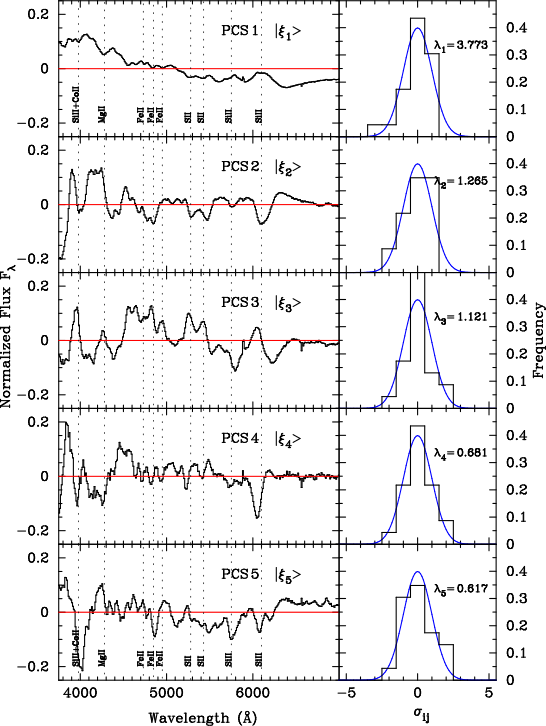
\includegraphics[angle=0,scale=0.8]{./figures/pca/20SNe_PCS_01to05_areanorm.ps}
%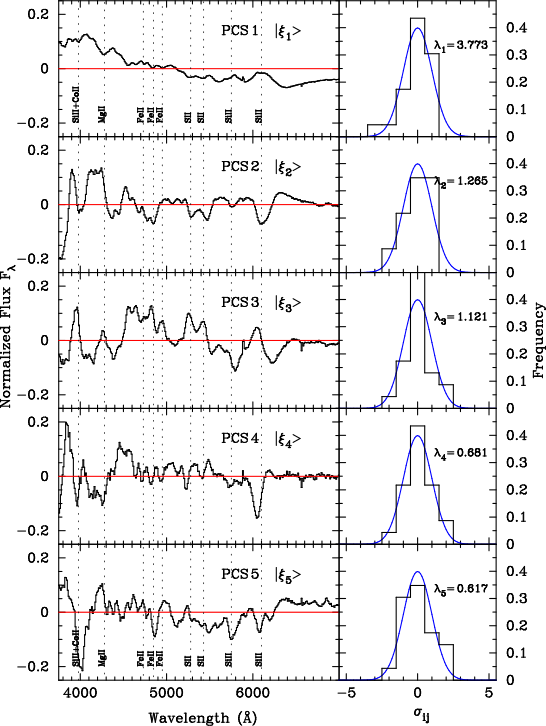
\includegraphics[angle=0,scale=0.4]{./figures/pca/20SNe_PCS_01to05_areanorm.ps}
%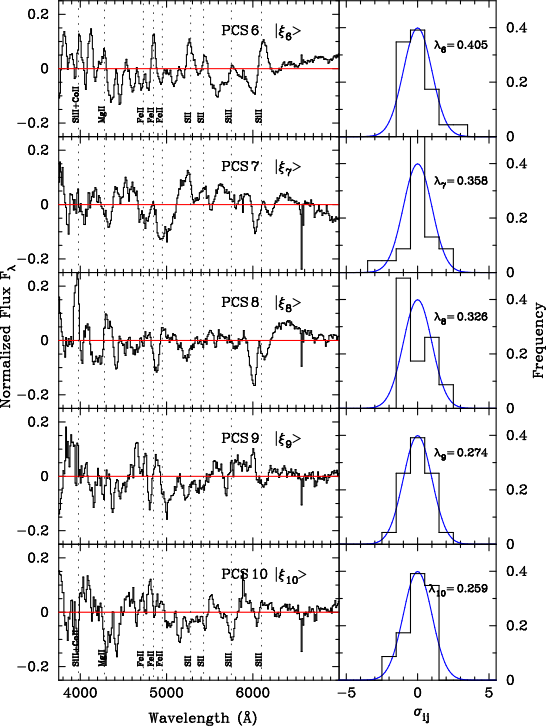
\includegraphics[angle=0,scale=0.4]{./figures/pca/20SNe_PCS_06to10_areanorm.ps}
\end{center}
\caption{
The first five eigenvectors, which account for 95.8\% of variation in the sample. Note the slope of the first eigenvector.
}
\label{fig:eigne1}
\end{figure}
\begin{figure}[htp]
\begin{center}
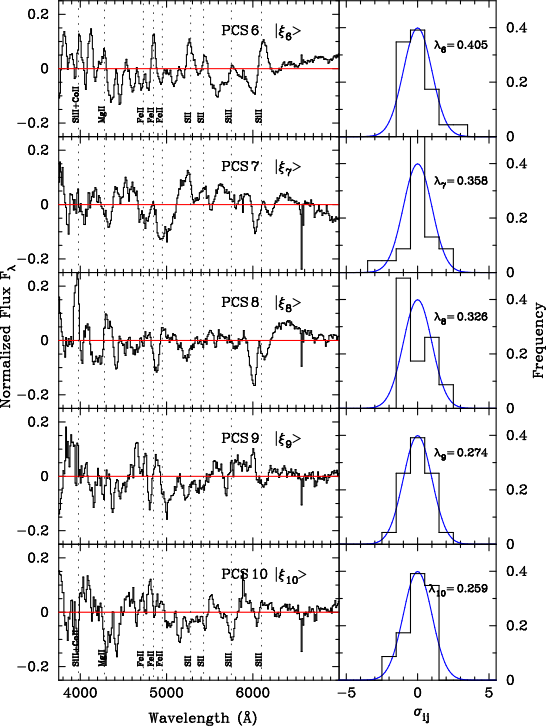
\includegraphics[angle=0,scale=0.8]{./figures/pca/20SNe_PCS_06to10_areanorm.ps}
\end{center}
\caption{
Eigenvectors six through ten, which account for 2.9\% of variation in the sample. 
}
\label{fig:eigen2}
\end{figure}
\begin{figure}[htp]
\begin{center}
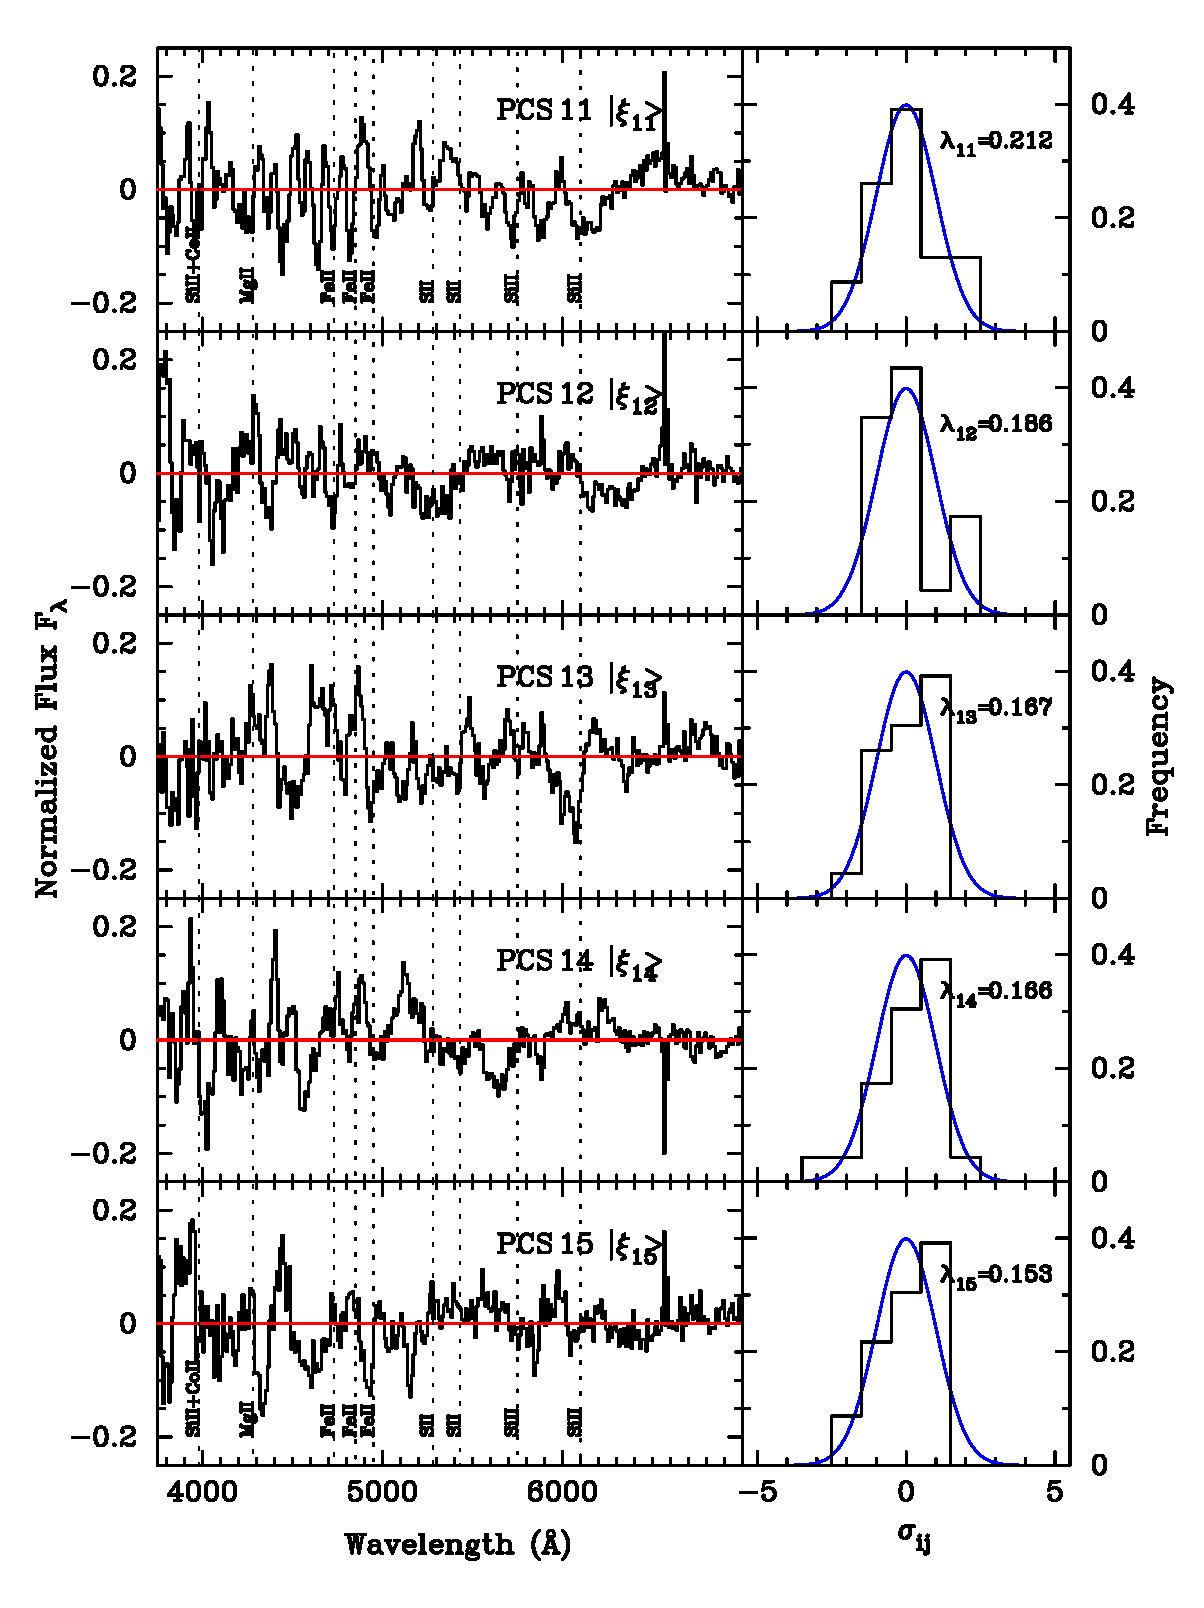
\includegraphics[angle=0,scale=0.8]{./figures/pca/20SNe_PCS_11to15_areanorm.ps}
\end{center}
\caption{
Eigenvectors eleven through fifteen, which account for 0.9\% of variation in the sample. 
}
\label{fig:eigen3}
\end{figure}
\begin{figure}[htp]
\begin{center}
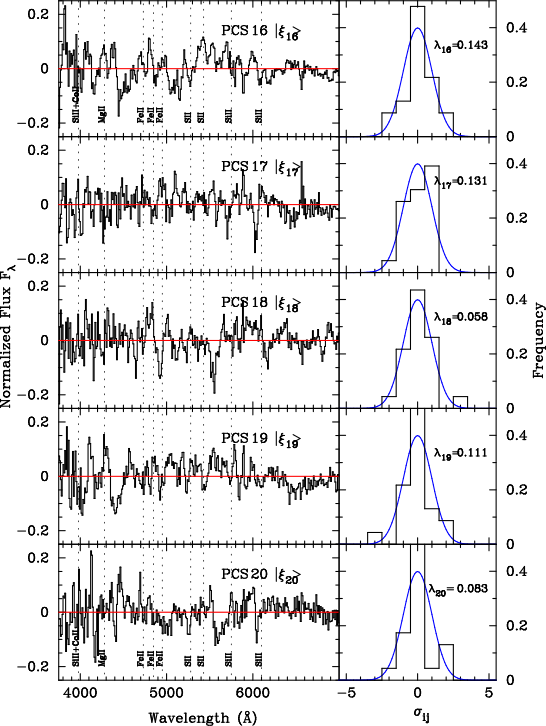
\includegraphics[angle=0,scale=0.8]{./figures/pca/20SNe_PCS_16to20_areanorm.ps}
\end{center}
\caption{
Eigenvectors sixteen through twenty, which account for 0.3\% of variation in the sample. 
}
\label{fig:eigen4}
\end{figure}


\begin{figure}[htp]
\begin{center}
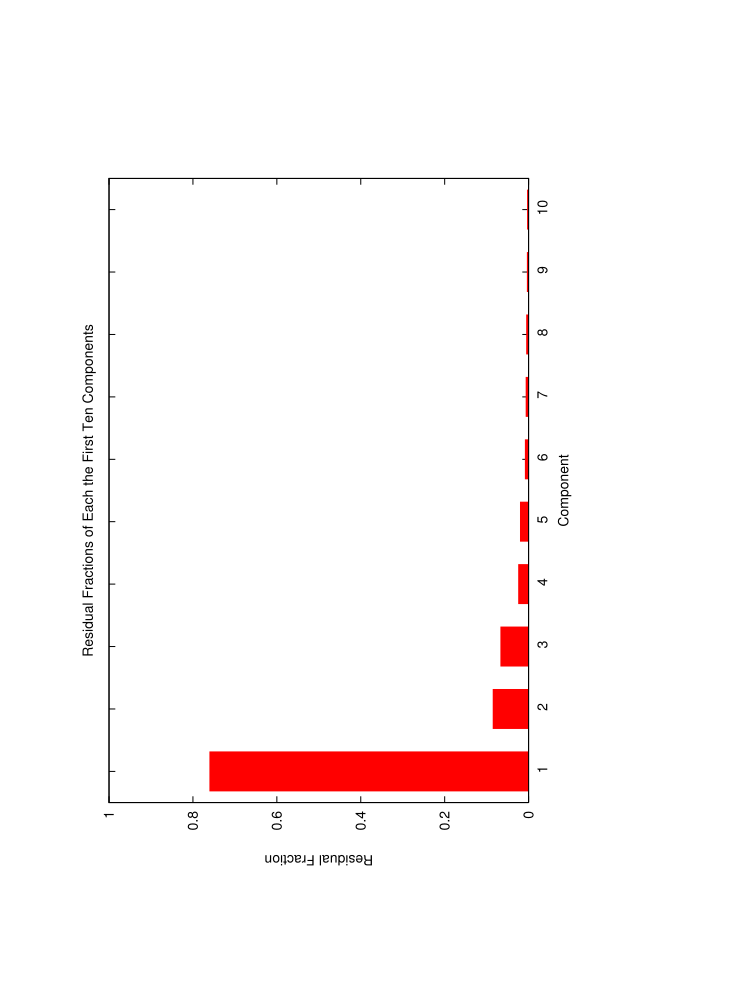
\includegraphics[angle=-90,scale=0.66]{./figures/hand_made/residual_fraction.ps}
\end{center}
\caption{
The residual fraction of the first ten components.
}
\label{fig:residualfrac1-5}
\end{figure}

% Built from SN_residual_fraction.dat
%% The values (usually only l,r and c) in the last part of
%% \begin{deluxetable}{} command tell LaTeX how many columns
%% there are and how to align them.
\begin{deluxetable}{ccccc}

%% Keep a portrait orientation

%% Over-ride the default font size
%% Use Default (12pt)

%% Use \tablewidth{?pt} to over-ride the default table width.
%% If you are unhappy with the default look at the end of the
%% *.log file to see what the default was set at before adjusting
%% this value.

%% This is the title of the table.
\tablecaption{Residual Fractions}

%% This command over-rides LaTeX's natural table count
%% and replaces it with this number.  LaTeX will increment 
%% all other tables after this table based on this number
\tablenum{5}

%% The \tablehead gives provides the column headers.  It
%% is currently set up so that the column labels are on the
%% top line and the units surrounded by ()s are in the 
%% bottom line.  You may add more header information by writing
%% another line between these lines. For each column that requries
%% extra information be sure to include a \colhead{text} command
%% and remember to end any extra lines with \\ and include the 
%% correct number of &s.
\tablehead{\colhead{Component} & \colhead{Eigenvalue} & \colhead{Eigenvalue$^{1/2}$} & \colhead{Fraction} & \colhead{Comulative Fraction} \\ 
\colhead{} & \colhead{$\lambda_{j}^{2}$} & \colhead{$\lambda_{j}$} & \colhead{} & \colhead{} } 

%% All data must appear between the \startdata and \enddata commands
\startdata
1 & 14.2425 & 3.7739 & 0.7606 & 0.7606 \\
2 & 1.6013 & 1.2654 & 0.0855 & 0.8461 \\
3 & 1.2576 & 1.1214 & 0.0672 & 0.9132 \\
4 & 0.4647 & 0.6817 & 0.0248 & 0.9380 \\
5 & 0.3816 & 0.6177 & 0.0204 & 0.9584 \\
6 & 0.1645 & 0.4056 & 0.0088 & 0.9672 \\
7 & 0.1284 & 0.3583 & 0.0069 & 0.9740 \\
8 & 0.1069 & 0.3269 & 0.0057 & 0.9798 \\
9 & 0.0755 & 0.2747 & 0.0040 & 0.9838 \\
10 & 0.0674 & 0.2596 & 0.0036 & 0.9874 \\
11 & 0.0452 & 0.2126 & 0.0024 & 0.9898 \\
12 & 0.0347 & 0.1862 & 0.0019 & 0.9916 \\
13 & 0.0282 & 0.1679 & 0.0015 & 0.9931 \\
14 & 0.0277 & 0.1664 & 0.0015 & 0.9946 \\
15 & 0.0237 & 0.1539 & 0.0013 & 0.9959 \\
16 & 0.0205 & 0.1432 & 0.0011 & 0.9970 \\
17 & 0.0173 & 0.1314 & 0.0009 & 0.9979 \\
18 & 0.0035 & 0.0590 & 0.0002 & 0.9981 \\
19 & 0.0124 & 0.1112 & 0.0007 & 0.9988 \\
20 & 0.0070 & 0.0839 & 0.0004 & 0.9991 \\
21 & 0.0083 & 0.0913 & 0.0004 & 0.9996 \\
22 & 0.0079 & 0.0891 & 0.0004 & 1.0000 \\
\enddata

%% Include any \tablenotetext{key}{text}, \tablerefs{ref list},
%% or \tablecomments{text} between the \enddata and 
%% \end{deluxetable} commands

%% No \tablecomments indicated

%% No \tablerefs indicated

\end{deluxetable}


The first eigenvector alone accounts for 76\% of variation in the data set. While the other eigenvectors are relatively flat, the first eigenvector has a definate slope. This allows it to account for differences in the color of supernovae spectra in the data set, with positive coeffecients creating bluer spectra and negative coefficents creating redder spectra. 

Eigenvectors two through five, which combined account for 19.8\% of variation, are all relatively flat. They primarily control the depths of different lines as well as the ratio of lines.

Eigenvectors six through twenty-two combined account for only 4.2\% of variation in the data set. They primarily appear to represent noise in the spectra, and so do not appear to be useful in classifying or categorizing supernovae.

\subsection{Classification of Supernovae}
$\sigma_{1}$ is primarily responsible for the color of a supernova. Supernova with $\sigma_{1} > 0$ are blue, while those with $\sigma_{1} < 0$ are red. $\sigma_{2}$ and $\sigma_{3}$ control the ratio of various absorption features. We have divided the supernovae into classes based on the values of their $\sigma_{1}$ and $\sigma_{2}$ normalized weights. 

We define a coordinate system such that:

$$ r_{i} = \sqrt( \sigma^{2}_{i1} + \sigma^{2}_{i2} )$$
$$ \tan{\theta_{i}} = \frac {\sigma_{i2}}{\sigma_{i1}} $$

Using this system, classes I-IV are defined by the the four quadrants. We define a class zero centered on the origin with a radius $r_{0}$ defined so that the probability of a supernova lying within it are $P = 0.2$. We solve for $r_{i}$ using:

$$ P(r \le r_{0}) = \int_{0}^{r_{0}} r e^{-r^{2}/2} dr = 1 -  e^{-r_{0}^{2}/2} $$

Class zero supernovae are the 20\% of the sample closest to the mean spectrum. Class I are those supernovae with $\sigma_{1} > 0$ and $\sigma_{2} > 0$. Class I are blue with sharp peaks and deep absorption lines. Class II supernovae are defined by $\sigma_{1} < 0$ and $\sigma_{2} > 0$. The have deep lines, but are red. Class III is defined by $\sigma_{1} > 0$ and $\sigma_{2} < 0$. These supernovae are red, with a spectrum that is more flat with less defined features. SN1991bg is a Class III supernova, nearly two standard deviations from the mean in both of its normalized weights. Class IV are those supernovae with $\sigma_{1} > 0$ and $\sigma_{2} < 0$. They are blue with less pronounced features. SN1991T is a Class IV supernova.

In order to visualize how $\sigma_{1}$ and $\sigma_{2}$ effect the shape of a type Ia spectrum, we have provided a plot of the mean spectrum (figure \ref{fig:classzero}), as well as the mean spectrum plus the first two components set so that we create a spectrum within each class, I through IV (figure \ref{fig:fourclasses}). For each of these four demonstration spectra the weights are one standard deviation from the mean.

\begin{figure}[ht]
\begin{center}
\includegraphics[angle=-90,scale=0.66]{./figures/hand_made/avg.ps}
\end{center}
\caption{
The mean spectrum, $\vec{\mu}$. Class zero are the 20\% of supernovae that are closest to this 
}
\label{fig:classzero}
\end{figure}

\begin{figure}[ht]
\begin{center}
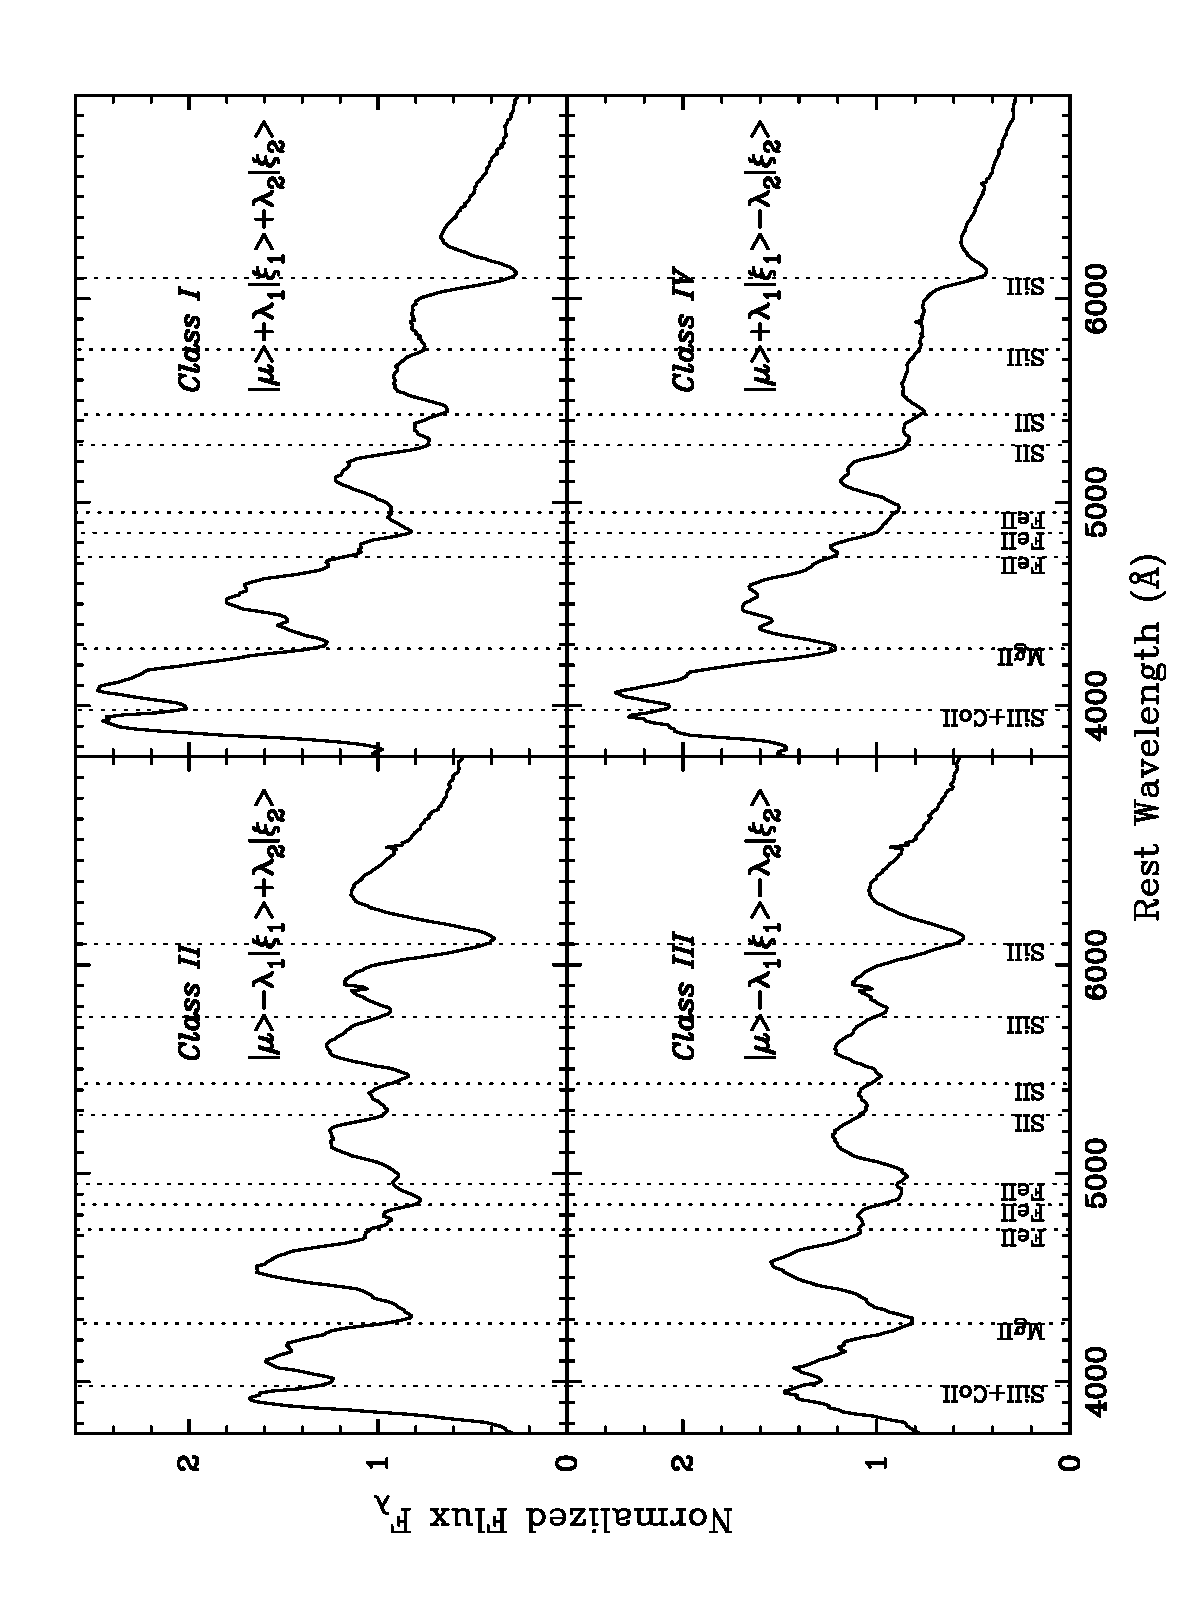
\includegraphics[angle=-90,scale=0.66]{./figures/pca/4class_areanorm.ps}
\end{center}
\caption{
Four spectra demonstrating Class I through Class IV, with the normalized weights set so that each one is one standard deviation from the norm.
}
\label{fig:fourclasses}
\end{figure}

\subsection{Color: Cardelli Law or Intrinsic?}
Although $E(B-V)$ has traditionally been attributed to extinction, recent work has suggested it may not be. For example, recent work by \citeauthor{conley08a} (\citeyear{conley08a}) has indicated that single parameter functions, such as dust laws, are in general unable to reproduce the variation in color seen in supernovae. They further find that the $U - B$ vs. $B - V$ relation found for their type Ia supernovae do not follow the relation one would expect for Milky-Way like dust.

% Conley fig
\begin{figure}[ht]
\begin{center}
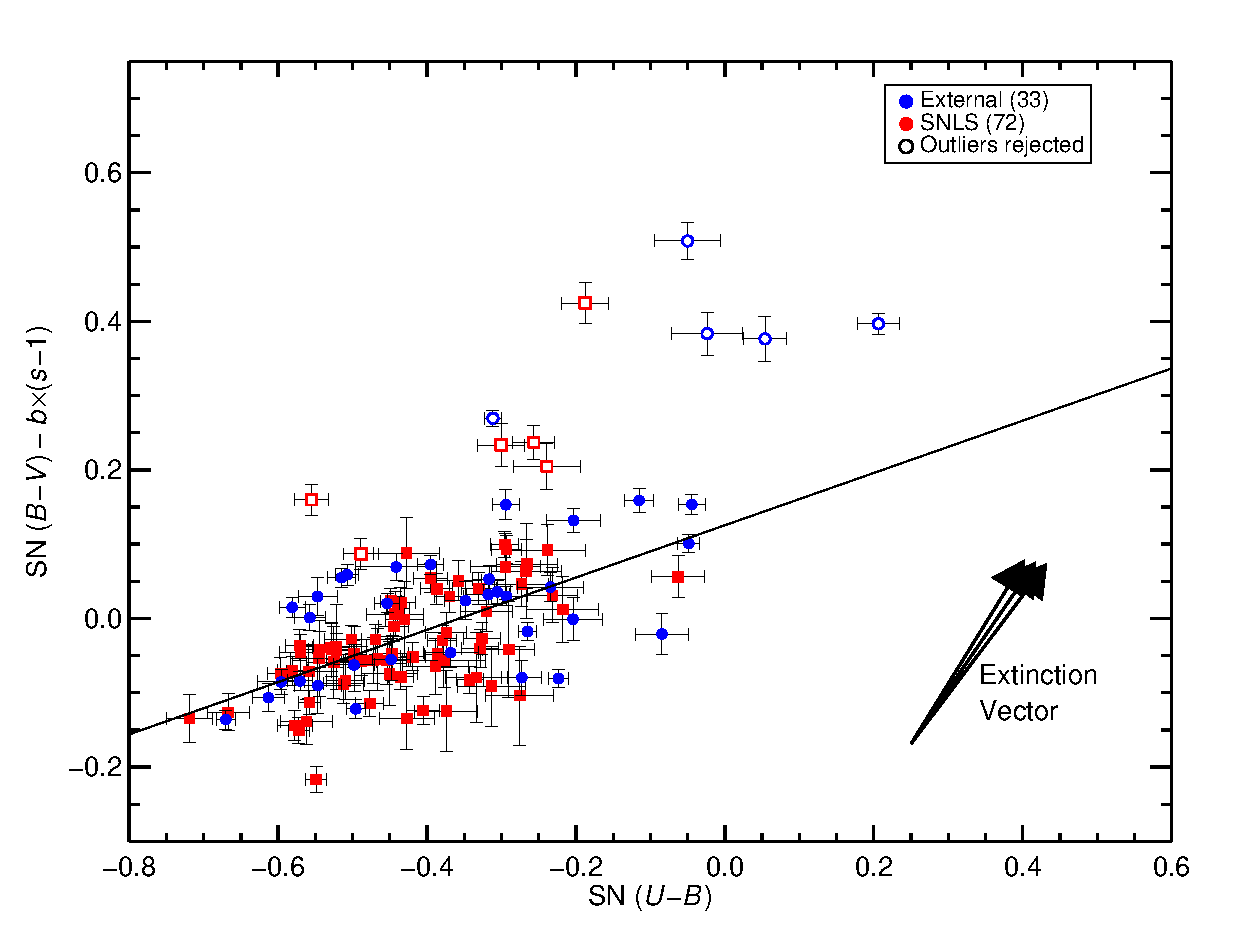
\includegraphics[angle=0,scale=0.8]{./figures/conley/f10_color.eps}
\end{center}
\caption{
The derived $U - B$ vs. $B - V$ relation found by \citeauthor{conley08a} (\citeyear{conley08a}). The best fit to the sample is the solid line. The arrow is the relation one would expect from Milky-Way like dust ($R_{v} = [1.6,3.1,4.6]$). Figure courtesy of \citeauthor{conley08a} (\citeyear{conley08a}).
}
\label{fig:conleyfigure}
\end{figure}

In line with the results of \citeauthor{conley08a} the first eigenvector suggests that color is partially an intrinsic quantity, and not simply due to extinction. If color is purely an extinction related-effect we would expect this eigenvector to be nearly featureless so that line ratios would be completely uncorrelated with color. However, we observe deviations from the first eigenvector that align with the MgII feature, the FeIII features and the SiII features. This suggests that color is, to some extent, correlated with spectral features and is therefore not entirely extinction but is intrinsic to each individual supernova. 

If the color excess observed in type Ia spectra was purely due to extinction then we should be able to use the Cardelli law \citep{cardelli89a} to account for it. We therefore attempt to warp the Hsiao template \citep{hsiao07a}, a template created by taking the mean spectra of over 100 type Ia supernovae near maximum light, with the Cardelli law. We fix $ R_{V} =3.1$ and vary $A_{V}$ until we find a minimum in the $\chi^{2}$ overlap between the warped Hsiao spectrum and the observed spectrum.

While many of the spectra appear to be able to be fit by a simple Cardelli law applied to the Hsiao template, nine supernovae fail. As expected the peculiar SN1991T and SN1991bg are not well fit. SN1998de, SN1998bp, SN1999cl, SN2000dk, and SN2000cx have spectral features that can not be matched with only a Cardelli law. SN1998aq and SN1999aa seem to fit well at first glance, but both have nonphysical preferred values of $A_{V}$, $-0.031$ for SN1998aq and $-0.062$ for SN1999aa. This suggests that for some of the supernovae Cardelli's law does not account for the observed color if $ R_{V} =3.1$ is fixed, however we can not say anything about the effects of letting $R_{V}$ float. This is something that we would like to explore in future work.

<<<<<<< .mine
<<<<<<< .mine
<<<<<<< .mine
<<<<<<< .mine
%%% The values (usually only l,r and c) in the last part of
%% \begin{deluxetable}{} command tell LaTeX how many columns
%% there are and how to align them.
\begin{deluxetable}{cc}

%% Keep a portrait orientation

%% Over-ride the default font size
%% Use Default (12pt)

%% Use \tablewidth{?pt} to over-ride the default table width.
%% If you are unhappy with the default look at the end of the
%% *.log file to see what the default was set at before adjusting
%% this value.

%% This is the title of the table.
\tablecaption{Result Of Warping Hsiao Template With Cardelli Law}

%% This command over-rides LaTeX's natural table count
%% and replaces it with this number.  LaTeX will increment
%% all other tables after this table based on this number
\tablenum{4}

%% The \tablehead gives provides the column headers.  It
%% is currently set up so that the column labels are on the
%% top line and the units surrounded by ()s are in the
%% bottom line.  You may add more header information by writing
%% another line between these lines. For each column that requries
%% extra information be sure to include a \colhead{text} command
%% and remember to end any extra lines with \\ and include the
%% correct number of &s.
\tablehead{\colhead{Well fit supernovae} & \colhead{Badly fit supernovae} \\
\colhead{} & \colhead{} } % for units

%% All data must appear between the \startdata and \enddata commands
\startdata
SN1997dt & SN1991T \\
SN1998aq & SN1991bg \\
SN1999dh & SN1998bp \\
SN1998V  & SN1998de \\
SN1998eg & 
SN1998ec & SN1999ac \\
SN1999aa & SN1999cc \\
SN1999dq & SN1999cl \\
SN1999gd & SN1999ej \\
SN1999gp & SN2000cx \\
SN2000cf & SN2000dk \\
SN2000fa \\
SN2000es
\enddata

%% Include any \tablenotetext{key}{text}, \tablerefs{ref list},
%% or \tablecomments{text} between the \enddata and
%% \end{deluxetable} commands

%% No \tablecomments indicated

%% No \tablerefs indicated

\end{deluxetable}


=======
Warping Hsiao's template with a Cardelli law provides a qualitative indication that color is not entirely due to extinction, but does not provide us with a quantitative method of determining the ammount of color excess due to extinction. For this we turn to our eigenvectors.
=======
Warping Hsiao's template with a Cardelli law provides a qualitative indication that color is not entirely due to extinction, but does not provide us with a quantitative method of determining the amount of color excess due to extinction. For this we turn to our eigenvectors.
=======
Warping Hsiao's template with a Cardelli law provides a qualitative indication that color is not entirely due to extinction, but it does not provide us with a quantitative method of determining the amount of color excess due to extinction. For this we turn to our eigenvectors.
=======
Warping Hsiao's template with a Cardelli law provides a qualitative indication that color is not entirely due to extinction, but it does not provide us with a quantitative method of determining the amount of color excess due to extinction. For this we turn to the eigenvectors.
>>>>>>> .r1177
>>>>>>> .r1139
>>>>>>> .r1130
>>>>>>> .r1097

In figures \ref{fig:sig1sig2}, \ref{fig:sig1sig3}, and \ref{fig:sig2sig3} we plot the normalized weight functions of the supernovae against each other. Supernovae with similar features will cluster. Further, it is possible to calculate a extinction vector in this space which allows us to observe exactly how much color excess is due to extinction. We plot the extinction vector by using the Cardelli law to warp the mean spectrum from the PCA. We fix $R_{V} = 3.1$ and increment $A_{V}$ by 0.2. We then normalize this spectrum by its area again and subtract off the mean spectrum. We then dot this with an eigenvector which gives us a weight. Mathematically this is:

$$ c_{j}^{CCM} = \vec{\xi_{j}} \cdot \left[ \frac {\vec{\mu} \cdot CCM(R_{V}=3.1,A_{V})}{Normalization} - \vec{\mu} \right] $$

Where $\vec{\mu}$ is the mean spectrum, $CCM(R_{V}=3.1,A_{V})$ is the Cardelli factor, and $\vec{\xi_{j}}$ is the $j$th eigenvector.

\begin{figure}[ht]
\begin{center}
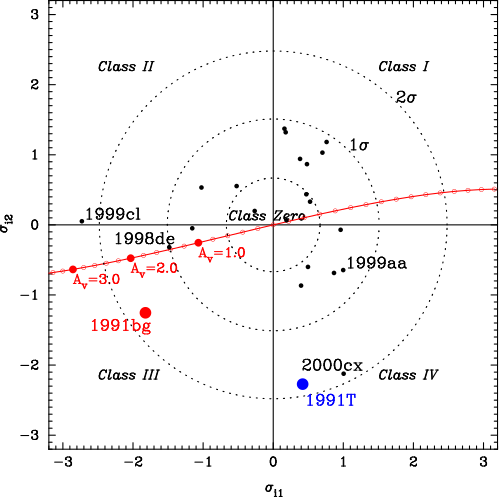
\includegraphics[angle=0,scale=0.8]{./figures/pca/sigma1_vs_sigma2_areanorm.ps}
\end{center}
\caption{
Supernovae plotted by their first and second normalized weight. Supernovae with $\sigma_{1} > 0$ are blue, while those with $\sigma_{1} < 0$ are red. The red line marks the expected extinction vector for Cardelli law extinction, with each open circle marking a step in $A_{V}$ of $0.2$.
}
\label{fig:sig1sig2}
\end{figure}

\begin{figure}[ht]
\begin{center}
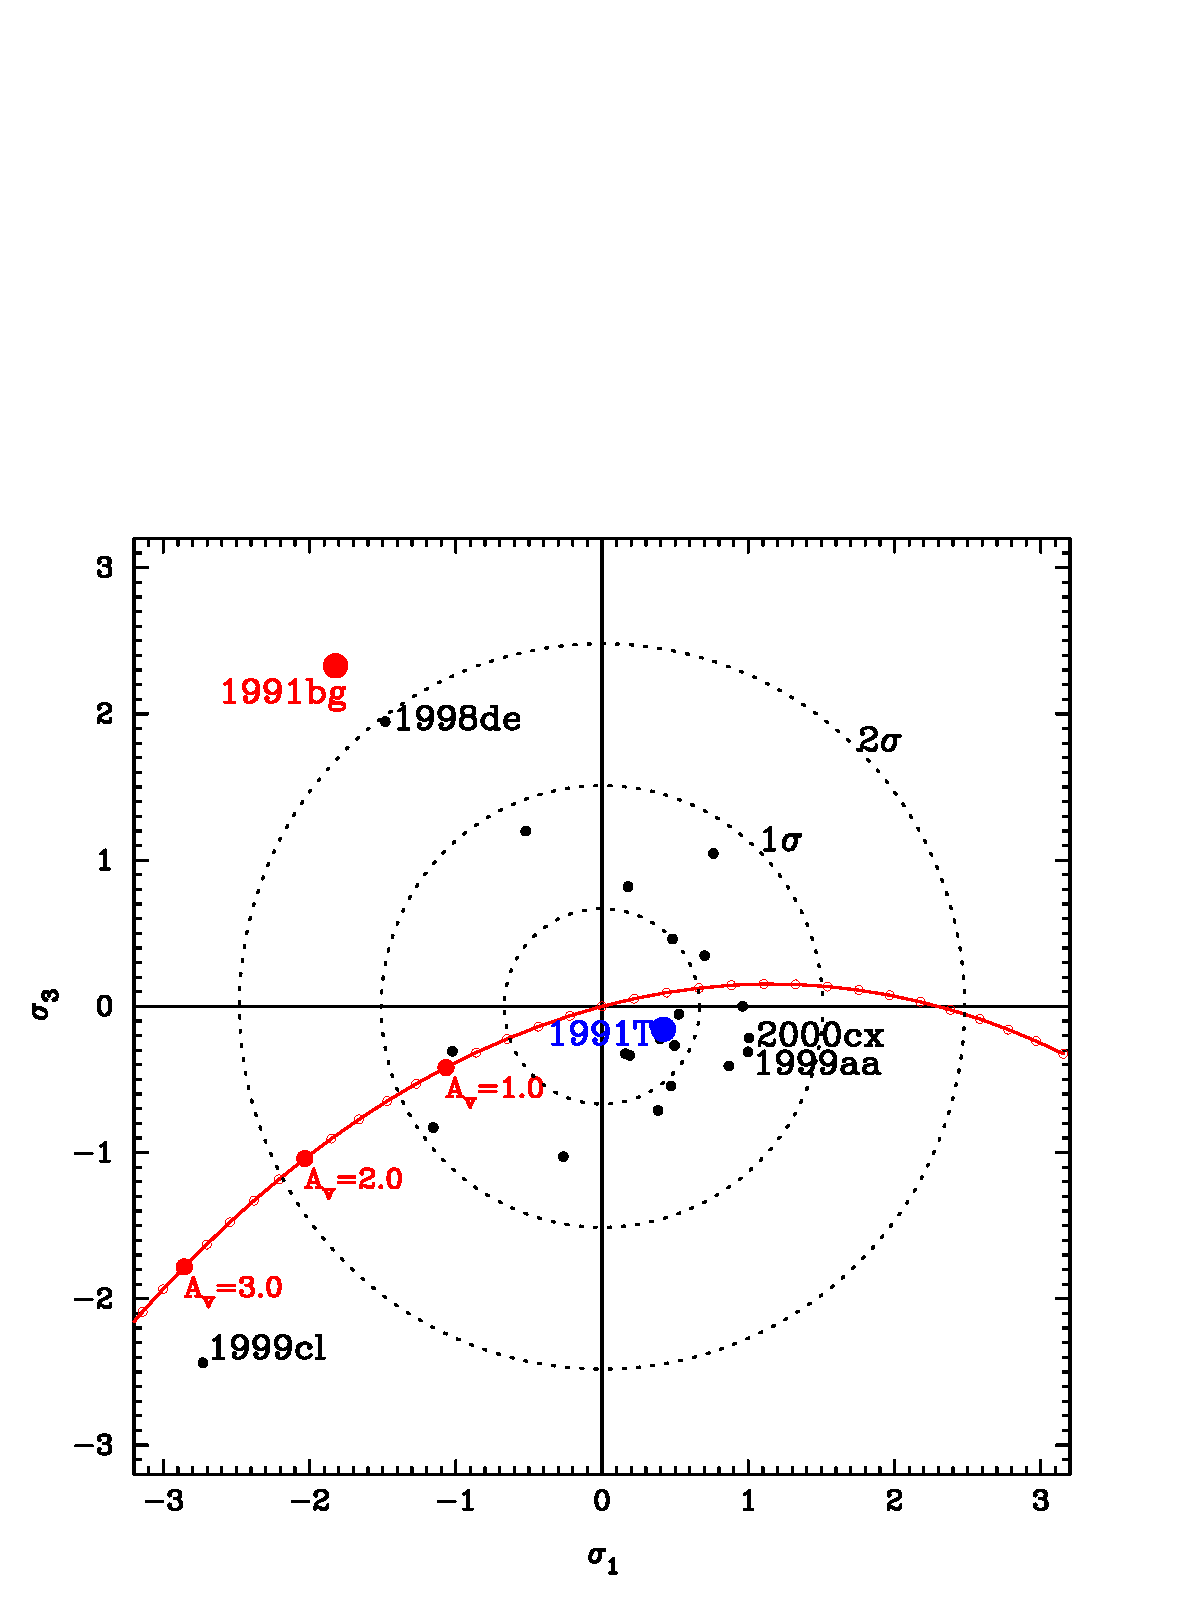
\includegraphics[angle=0,scale=0.8]{./figures/pca/sigma1_vs_sigma3_areanorm.ps}
\end{center}
\caption{
Supernovae plotted by their first and third normalized weight. Supernovae with $\sigma_{1} > 0$ are blue, while those with $\sigma_{1} < 0$ are red. The red line marks the expected extinction vector for Cardelli law extinction, with each open circle marking a step in $A_{V}$ of $0.2$.
}
\label{fig:sig1sig3}
\end{figure}

\begin{figure}[ht]
\begin{center}
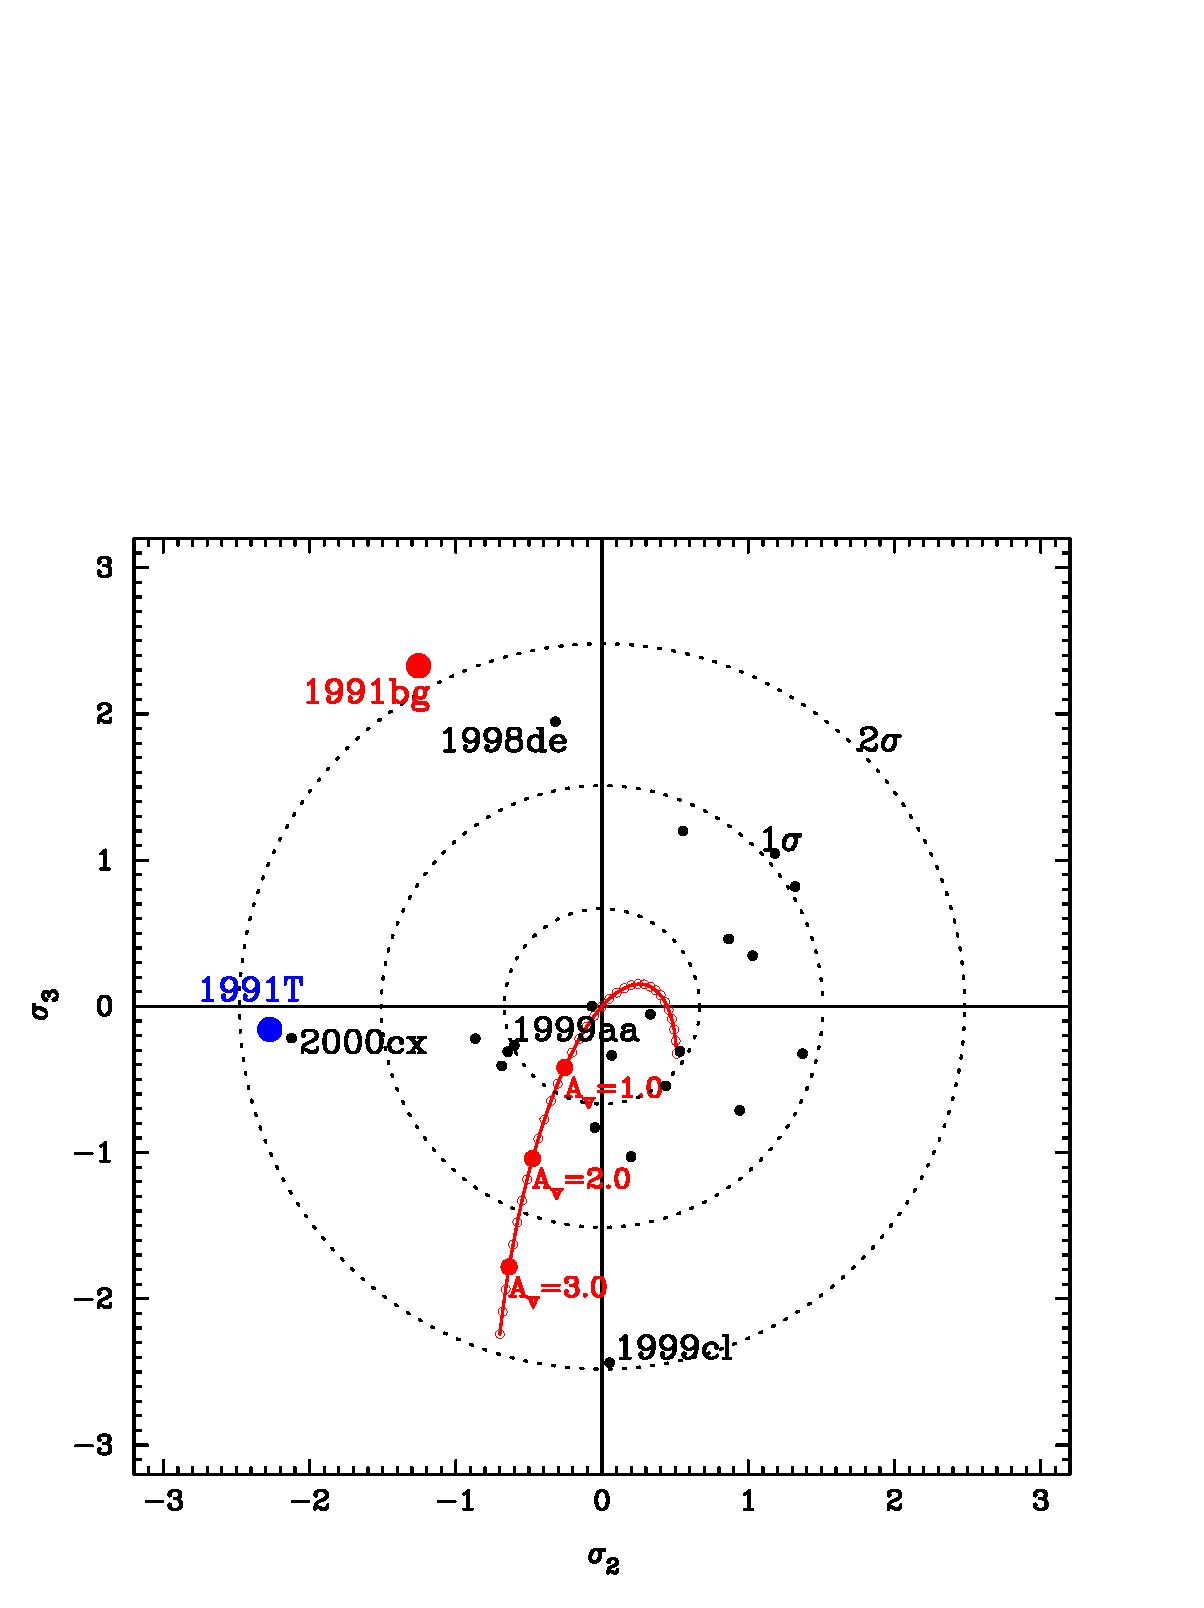
\includegraphics[angle=0,scale=0.8]{./figures/pca/sigma2_vs_sigma3_areanorm.ps}
\end{center}
\caption{
Supernovae plotted by their second and third normalized weight. The red line marks the expected extinction vector for Cardelli law extinction, with each open circle marking a step in $A_{V}$ of $0.2$.
}
\label{fig:sig2sig3}
\end{figure}

Only if a supernova lies near the extinction line, in all three plots, is its color due to Cardelli like dust. It is worth nothing that very few supernovae lie close to the extinction vector in all three plots. This suggests that the variation we see in color from most type Ia supernovae is due to intrinsic properties of the supernovae and not extinction.

\clearpage
\subsection{Applications to the Hubble Diagram}
We hope the PCA eigenvectors will assist in future cosmology research involving type Ia supernovae. In order to get an idea of their usefulness, we create a series of Hubble diagrams with the supernovae from the data set, except for SN1991T and SN1991T as they do not have light curves and SN1999cl which was such an outlier that it badly pulled the fit. We plot $cz$ of the host galaxies of each of the supernovae against their maximum B band magnitude. Because the supernovae are nearby, they have peculiar velocity that must be corrected for. We used the $cz$ calculated relative to the cosmic microwave background \citep{fixsen96a}. We plot the Hubble law using $H_{0} = 71.9 km/s/Mpc$ as reported by \citet{hinshaw08a}.

We also make Hubble diagrams using color corrections (\citeauthor{astier06a} \citeyear{astier06a}; \citeauthor{sullivan03a} \citeyear{sullivan03a}), stretch corrections (\citeauthor{perlmutter97a} \citeyear{perlmutter97a}; \citeauthor{perlmutter99a} \citeyear{perlmutter99a}; \citeauthor{knop03} \citeyear{knop03}), and both color and stretch corrections combined. For these corrections we fit for $\alpha$ and $\beta$ iteratively, seeding with values of $\alpha = -1.24$ and $\beta = 2.28$ as determined by \citet{kowalski08a}. We find that for this sample, $\alpha = -2.084$ and $\beta = 3.610$. In order to find a fit that would correct most of our supernova, we removed by hand a single outlier with color $> 1$.

We then attempt to find a correlation between the normalized weights and dispersion around the Hubble line. While we'd like to be able to measure the effect on intrinsic dispersion, we do not have accurate enough error bars to do so. We plot the first normalized weight, $\sigma_{1}$ against $mag_{B} - Model$ and fit for a correction using weighted least squares. We then apply this correction and plot $\sigma_{2}$ against $mag_{B} - Model - A_{1}*\sigma_{1} - B_{1}$ where $A_{1}$ and $B_{1}$ are the slope and intercept of the correction. We continue to do this for the first five normalized weights. We then create Hubble diagrams using only the $\sigma_{1}$ correction, using $\sigma_{1}$ and $\sigma_{2}$, and so on until we use all of the corrections up to $\sigma_{5}$.

We then attempt to combine color, stretch, and the normalized weights into one correction. We use the same method as before, except we start by plotting $\sigma_{1}$ against $mag_{B} - Model - \alpha (S - 1) - \beta C$ which is the magnitudes already corrected with color and stretch. We repeat the above process, subtracting off corrections for each normalized weight found previously, before fitting a new correction for the next normalized weight.

We now have fourteen Hubble diagrams. Four were made with the uncorrected data, with color corrections, with stretch corrections, and with color and stretch corrections. Five were made with just using the normalized weights, and five were made combing color, stretch, and then using the normalized weights. For each of these Hubble Diagrams we calculate the dispersion, and then use this dispersion to remove any supernovae that are more than two standard deviations from the Hubble line, what we call a 2$\sigma$-cut dispersion. The supernova cut are marked by an $^{*}$ on table 6.

While table 6 seems to indicate that without using the 2$\sigma$-cut, we are able to achieve a lower dispersion with just our first weight than with color, stretch, or color and stretch combined corrections, this is without outlier rejection. If we reject SN1999cl, a four $\sigma$ outlier, and then perform the analysis, we find that the weight correction only improves the dispersion more than color alone, while stretch corrections and color with stretch corrections combined improve it more than using on the first weight. Using more than just the first weight increases dispersion, which is unexpected as PCA is guaranteed to lower dispersion. We see this increased dispersion though because we do not use the exact corrections determined by the PCA, but used a shortcut of fit for the corrections (the $A_{1}$ and $B_{1}$ mentioned above). Future analysis will be done with the PCA determined corrections.

If we apply the 2$\sigma$-cut after rejecting SN1999cl, we find that only using the first normalized weight gets us a dispersion that is lower than using a color correction alone or a stretch correction alone, but is worse than using a stretch correction and color correction combined. Again using more than just the first normalized weight increases the dispersion. Using color, stretch, and the first normalized weight increases dispersion as compared to using just color and stretch alone.

\clearpage
\begin{deluxetable}{ccccccccc}
\tablecaption{Distance From The Hubble Line In Magnitudes}
\tablenum{6}
\tablehead{\colhead{Supernova} & \colhead{Uncorrected} & \colhead{C} & \colhead{S} & \colhead{CS} & \colhead{W1}  & \colhead{W2} & \colhead{W3} & \colhead{CSW1}}
\startdata
SN1997dt & 2.734$^{*}$ & 2.537$^{*}$ & 0.716 & 0.519 & 1.169$^{*}$ & 0.487 & -0.062 & 1.185$^{*}$ \\
SN1998V & 0.074 & 0.010 & -0.054 & -0.118 & -0.294 & -1.130$^{*}$ & -1.446$^{*}$ & -0.217 \\
SN1998aq & 0.286 & 0.123 & 0.732 & 0.569 & 0.227 & -0.448 & -0.747 & 0.272 \\
SN1998bp & 1.503 & 0.962 & 0.530 & -0.012 & 0.389 & -0.536 & -0.476 & 0.367 \\
SN1998de & 2.678$^{*}$ & 2.275$^{*}$ & 0.535 & 0.132 & 0.880 & 0.305 & 0.590 & 0.947 \\
SN1998dh & 0.628 & 0.414 & 0.158 & -0.055 & -0.001 & -1.256$^{*}$ & -1.653$^{*}$ & 0.013 \\
SN1998ec & 0.741 & 0.700 & 0.111 & 0.070 & -0.190 & -0.973 & -1.581$^{*}$ & 0.331 \\
SN1998eg & 0.424 & 0.236 & 0.282 & 0.094 & 0.180 & -0.937 & -1.133 & -0.084 \\
SN1998es & 0.093 & 0.191 & -0.154 & -0.055 & -0.297 & -0.758 & -1.139 & -0.140 \\
SN1999aa & -0.022 & 0.074 & 0.119 & 0.215 & -0.054 & -0.497 & -0.890 & -0.099 \\
SN1999ac & 0.374 & 0.351 & -0.030 & -0.054 & -0.027 & -1.078 & -1.239 & -0.132 \\
SN1999cc & 0.484 & 0.098 & 0.328 & -0.058 & 0.013 & -1.068 & -1.581$^{*}$ & -0.092 \\
SN1999cl & 1.339 & 1.161 & -2.992$^{*}$ & -3.169$^{*}$ & -1.346$^{*}$ & -2.069$^{*}$ & -3.100$^{*}$ & -1.787$^{*}$ \\
SN1999dq & -0.071 & 0.044 & -0.493 & -0.378 & -0.530 & -0.884 & -1.251 & -0.418 \\
SN1999ej & 0.964 & 0.610 & 0.826 & 0.473 & 0.356 & -0.373 & -0.773 & 0.527 \\
SN1999gd & 1.638$^{*}$ & 1.506$^{*}$ & -0.058 & -0.190 & 0.168 & -0.749 & -1.141 & 0.416 \\
SN1999gp & 0.134 & 0.475 & -0.088 & 0.252 & 0.009 & -0.418 & -0.840 & -0.001 \\
SN2000cf & 0.381 & 0.208 & 0.346 & 0.173 & 0.180 & -0.998 & -0.984 & -0.033 \\
SN2000cx & 0.077 & -0.269 & 0.321 & -0.026 & 0.049 & 0.201 & -0.164 & -0.342 \\
SN2000dk & 0.471 & -0.017 & 0.230 & -0.258 & -0.145 & -1.379$^{*}$ & -1.433$^{*}$ & -0.198 \\
SN2000fa & 0.307 & 0.236 & 0.031 & -0.041 & -0.100 & -0.978 & -1.441$^{*}$ & -0.114 \\
\hline
Dispersion & 0.779 & 0.709 & 0.737 & 0.711 & 0.471 & 0.562 & 0.697 & 0.552 \\
2$\sigma$-cut & 0.419 & 0.341 & 0.319 & 0.237 & 0.291 & 0.464 & 0.497 & 0.322 \\
\enddata
\tablecomments{ C has been color corrected, S has been stretch corrected, CS has been color and stretch corrected, W1 has had a correction from the first normalized weight, W2 uses a correction from the first and second normalized weights, W3 uses a correction from the first, second, and third normalized weights. CSW1 uses a color and stretch correction, as well as corrections from the first normalized weight. The Dispersion is calculated as the standard deviation of the entries. 2$\sigma$-cut is the dispersion recalculated with supernovae that are more than two standard deviations from the Hubble line dropped. Entries marked with a $^{*}$ were dropped for the 2$\sigma$-cut calculation.}
\end{deluxetable}

\clearpage
\begin{deluxetable}{ccccccccc}
\tablecaption{Distance From The Hubble Line In Magnitudes}
\tablenum{7}
\tablehead{\colhead{Supernova} & \colhead{Uncorrected} & \colhead{C} & \colhead{S} & \colhead{CS} & \colhead{W1}  & \colhead{W2} & \colhead{W3} &\colhead{CSW1}}
\startdata
SN1997dt & 2.734$^{*}$ & 2.537$^{*}$ & 0.716$^{*}$ & 0.519$^{*}$ & 1.169$^{*}$ & 0.487 & -0.062 & 1.185$^{*}$ \\
SN1998V & 0.074 & 0.010 & -0.054 & -0.118 & -0.294 & -1.130$^{*}$ & -1.446$^{*}$ & -0.217 \\
SN1998aq & 0.286 & 0.123 & 0.732$^{*}$ & 0.569$^{*}$ & 0.227 & -0.448 & -0.747 & 0.272 \\
SN1998bp & 1.503 & 0.962 & 0.530 & -0.012 & 0.389 & -0.536 & -0.476 & 0.367 \\
SN1998de & 2.678$^{*}$ & 2.275$^{*}$ & 0.535 & 0.132 & 0.880$^{*}$ & 0.305 & 0.590 & 0.947$^{*}$ \\
SN1998dh & 0.628 & 0.414 & 0.158 & -0.055 & -0.001 & -1.256$^{*}$ & -1.653$^{*}$ & 0.013 \\
SN1998ec & 0.741 & 0.700 & 0.111 & 0.070 & -0.190 & -0.973 & -1.581$^{*}$ & 0.331 \\
SN1998eg & 0.424 & 0.236 & 0.282 & 0.094 & 0.180 & -0.937 & -1.133$^{*}$ & -0.084 \\
SN1998es & 0.093 & 0.191 & -0.154 & -0.055 & -0.297 & -0.758 & -1.139$^{*}$ & -0.140 \\
SN1999aa & -0.022 & 0.074 & 0.119 & 0.215 & -0.054 & -0.497 & -0.890 & -0.099 \\
SN1999ac & 0.374 & 0.351 & -0.030 & -0.054 & -0.027 & -1.078$^{*}$ & -1.239$^{*}$ & -0.132 \\
SN1999cc & 0.484 & 0.098 & 0.328 & -0.058 & 0.013 & -1.068$^{*}$ & -1.581$^{*}$ & -0.092 \\
SN1999dq & -0.071 & 0.044 & -0.493 & -0.378 & -0.530 & -0.884 & -1.251$^{*}$ & -0.418 \\
SN1999ej & 0.964 & 0.610 & 0.826$^{*}$ & 0.473 & 0.356 & -0.373 & -0.773 & 0.527 \\
SN1999gd & 1.638$^{*}$ & 1.506$^{*}$ & -0.058 & -0.190 & 0.168 & -0.749 & -1.141$^{*}$ & 0.416 \\
SN1999gp & 0.134 & 0.475 & -0.088 & 0.252 & 0.009 & -0.418 & -0.840 & -0.001 \\
SN2000cf & 0.381 & 0.208 & 0.346 & 0.173 & 0.180 & -0.998$^{*}$ & -0.984 & -0.033 \\
SN2000cx & 0.077 & -0.269 & 0.321 & -0.026 & 0.049 & 0.201 & -0.164 & -0.342 \\
SN2000dk & 0.471 & -0.017 & 0.230 & -0.258 & -0.145 & -1.379$^{*}$ & -1.433$^{*}$ & -0.198 \\
SN2000fa & 0.307 & 0.236 & 0.031 & -0.041 & -0.100 & -0.978 & -1.441$^{*}$ & -0.114 \\
\hline
Dispersion & 0.785 & 0.713 & 0.319 & 0.237 & 0.371 & 0.493 & 0.551 & 0.396 \\
2$\sigma$-cut & 0.374 & 0.283 & 0.247 & 0.187 & 0.224 & 0.451 & 0.461 & 0.254 \\
\enddata
\tablecomments{ The same as table 6, but SN1999cl has been removed before any calculations.}
\end{deluxetable}

\clearpage

\begin{figure}[ht]
\begin{center}
\includegraphics[angle=-90,scale=0.66]{./figures/hand_made/01_hubble.ps}
\end{center}
\caption{
Hubble diagram of uncorrected supernovae.
}
\label{fig:hduncor}
\end{figure}
\clearpage

\begin{figure}[ht]
\begin{center}
\includegraphics[angle=-90,scale=0.66]{./figures/hand_made/02_hubble_stretch_corrected.ps}
\end{center}
\caption{
Hubble diagram of stretch corrected supernovae.
}
\label{fig:hds}
\end{figure}
\clearpage

\begin{figure}[ht]
\begin{center}
\includegraphics[angle=-90,scale=0.66]{./figures/hand_made/03_hubble_color_corrected.ps}
\end{center}
\caption{
Hubble diagram of color corrected supernovae.
}
\label{fig:hdc}
\end{figure}
\clearpage

\begin{figure}[ht]
\begin{center}
\includegraphics[angle=-90,scale=0.66]{./figures/hand_made/04_hubble_color_stretch_corrected.ps}
\end{center}
\caption{
Hubble diagram of color and stretch corrected supernovae.
}
\label{fig:hdcs}
\end{figure}
\clearpage

\begin{figure}[ht]
\begin{center}
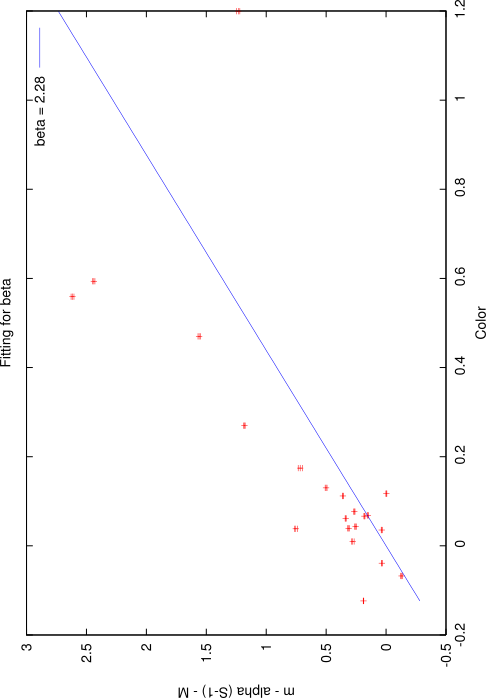
\includegraphics[angle=-90,scale=0.66]{./figures/hand_made/05_hubble_beta.ps}
\end{center}
\caption{
$\beta=3.610$, and the supernovae.
}
\label{fig:beta}
\end{figure}
\clearpage

\begin{figure}[ht]
\begin{center}
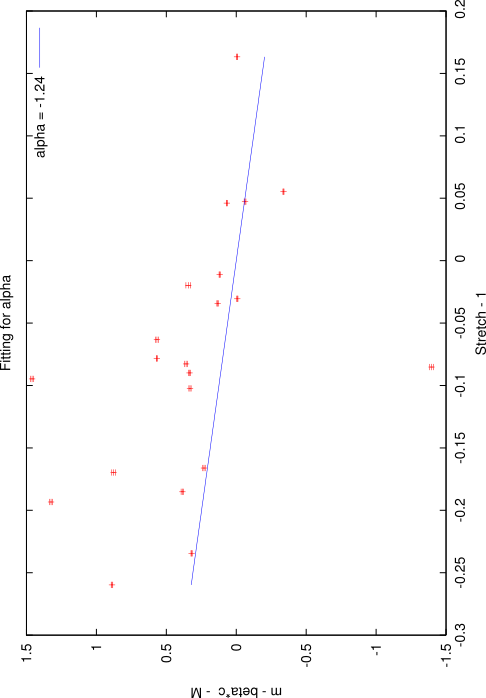
\includegraphics[angle=-90,scale=0.66]{./figures/hand_made/06_hubble_alpha.ps}
\end{center}
\caption{
$\alpha = -2.084$, and the supernovae.
}
\label{fig:alpha}
\end{figure}
\clearpage

\begin{figure}[ht]
\begin{center}
\includegraphics[angle=-90,scale=0.66]{./figures/hand_made/07_hubble_sig_corrected.ps}
\end{center}
\caption{
Hubble diagram of first normalized weight corrected supernovae.
}
\label{fig:hdw}
\end{figure}
\clearpage

\begin{figure}[ht]
\begin{center}
\includegraphics[angle=-90,scale=0.66]{./figures/hand_made/08_hubble_color_stretch_sig_corrected.ps}
\end{center}
\caption{
Hubble diagram of color, stretch, and first normalized weight corrected supernovae.
}
\label{fig:hdcsw}
\end{figure}
\clearpage

\section{Conclusion}

We find that using only the first five eigenvectors we are able to represent 95.8\% of diversity within the supernova sample. It is no longer necessary to make qualitative judgments such as "SN1991T-like" when classifying supernovae; using the PCA components supernovae can be quantitatively classified into five types.

The first eigenvector has a non-zero slope which allows it to account for color. However, it also contains spectral features indicating a correlation between absorption lines and color. This suggests that color variation is not purely due to Cardelli like dust, but is partially intrinsic. We explored this possibility by warping Hsiao's template using Cardelli's law to attempt to match the supernovae and found that in many cases this does not adequately fit the spectra. We then plotted the normalized weights of the supernovae against each other along with a vector representing the normalized weights we calculated for an average spectrum warped by Cardelli dust and found that very few of the supernovae fell along this vector. We therefore conclude that color variation is primarily intrinsic.

We attempt to correlate the normalized weights with dispersion around the Hubble line. When a cut is not applied, we are able to improve the dispersion around the Hubble line by using either just the first normalized weight, or by using color, stretch, and the first normalized weight. If a 2$\sigma$ cut is applied, we are unable to improve the dispersion using the normalized weights. However, the method of PCA requires only a single spectrum near maximum. Using this single spectrum we are able to improve the dispersion by 13\% compared to applying no corrections. In contrast, using a color and stretch correction improves upon the normalized weights method by 6\%, but requires a full, multiband lightcurve.

We've shown that PCA is useful in classifying type Ia supernovae in a quantitative manner and have used our results to argue that color excess in type Ia supernovae is intrinsic. We have also shown that PCA shows promise for reducing dispersion around the Hubble line. There are a few refinements one could do to improve this work in the future. On the data side having more supernovae would improve the quality of the components. Likewise, it has been suggested that SN1991bg does not fall on a continuum of type Ia supernovae and so removing it and other supernovae like SN1991bg before hand would likely improve the usefulness of the components for comparing and correcting more average type Ia supernovae.

We attempted to flux correct the supernovae, but the method we employed did not always improve the color. Exploring different methods of correction could improve the quality of the spectra used in the final PCA and would therefore improve the components. 

Our analysis could be improved in a few ways. First, when applying the Cardelli law to Hsiao's template, we fixed $R_{V}$. Allowing this to float would provide a more complete test of whether any type of Cardelli dust can account for reddening.  Second, we encountered problems with the Hubble diagrams and the dispersion corrections. This is partially due to the fact that many of the supernovae have peculiar velocities that we did not correct for. One could correct for these by account for Virgo infall, the pull of the Great Attractor, and other local effects, or one could use higher redshift supernovae where peculiar velocity becomes unimportant. Further, the method we used to calculate the weight corrections for dispersion did not take advantage of the fact that the eigenvectors are orthonormal. It is possible to do this and get a result where the dispersion is always lowered. This method will be persued in future analysis.

\section{Acknowledgments}
Many people helped in the process of writing this thesis, without them it would have never been completed. I would like to thank Saul Perlmutter for allowing me to work with his group, The Supernova Cosmology Project, for the past two and a half years and for giving me an exciting and informative look into the day to day workings of a observational cosmology group. Working with Professor Perlmutter has made it clear to me that research physics is my future. I would also like to thank Nao Suzuki, who guided me when I first joined the SCP and who was always free to answer any questions I had about cosmology or my thesis. I am grateful to Mark Strovink who suggested a few ways to improve upon the methods laid out in this thesis, and am also grateful for the time David Rubin spent explaining Hubble diagrams, intrinsic dispersion, and how to get SALT2 to work. Lastly, I'd like to thank the entire SCP for their support, having so many knowledgeable people around me made writing this thesis much easier.


%\outlineend{draft}

% Bibliography
\clearpage % Dump all charts BEFORE refs
\bibliographystyle{../../papers/00_bibdatabase/apj}
\bibliography{../../papers/00_bibdatabase/archive}

% Figures
\clearpage % clearpage to makesure all tables/figures have been dumped BEFORE these
\section*{Appendix: A}
With the exception of SN1991T and SN1991bg, we provide four figures for each supernova used in this analysis. The first figure shows a blue spectrum, and possibly a red spectrum. If there is only a blue spectrum, then we applied no flux correction to the raw data, and only re-binned it and trimmed the edges off before using it in our analysis. If we show a red and a blue spectrum, then the red spectrum represents the data before flux calibration, and the blue spectrum shows the data we finally used after flux calibration.

The second figure shows a step in our flux calibration process. We fit a light curve with SALT2 and used SALT2 to generate an artificial spectrum for the supernova. We then re-binned both the supernova's spectrum and the SALT2 spectrum to 500 \AA\ bins. We compared these, and plotted a point for each bin which represents the number we'd have to multiple the data bin by to match the SALT2 bin. If a pink line is shown, then this is the function we used for the flux calibration. If no line is shown, then no flux calibration was performed.

The third figure shows the light curve fit by SALT2. The x scale of this plot is adjusted to only include the portion that SALT2 fit. While other points exist they are not included in the fit and so are not plotted.

The fourth figure shows the supernova spectrum, and the best fit using a $\chi^{2}$ fit of Hsiao's template warped with a Cardelli law. These plots were created to give an indication of the inability of a single parameter warp to account for all of a supernova's features.



\begin{figure}[p]
\centering
\includegraphics[angle=-90,width=0.8\textwidth]{./figures/spectrabeforeafter/SN1997dt_handpicked_v001_v027_before_after_spectra.ps}
\hfill
\includegraphics[angle=-90,width=0.8\textwidth]{./figures/corrections/SN1997dt_v001_correction.ps}
\hfill
\caption{SN1997dt spectrum before and after warping, as well as the correction function used to warp.}
\label{fig:SN1997dtfour1}
\end{figure}

\clearpage

\begin{figure}[p]
\centering
\includegraphics[angle=-90,width=0.8\textwidth]{./figures/ltcv/SN1997dt_v027_lightcurve.ps}
\hfill
\includegraphics[angle=-90,width=0.8\textwidth]{./figures/hsiao/SN1997dt_v001_hsiao.ps}
\hfill
\caption{SN1997dt light curve fit, as well as the best fit for Hsiao template warped using the Cardelli law to match the spectrum.}
\label{fig:SN1997dtfour2}
\end{figure}

\clearpage

\begin{figure}[p]
\centering
\includegraphics[angle=-90,width=0.8\textwidth]{./figures/spectrabeforeafter/SN1998V_handpicked_v001_v023_before_after_spectra.ps}
\hfill
\includegraphics[angle=-90,width=0.8\textwidth]{./figures/corrections/SN1998V_v001_correction.ps}
\hfill
\caption{SN1998V spectrum before and after warping, as well as the correction function used to warp.}
\label{fig:SN1998Vfour1}
\end{figure}

\clearpage

\begin{figure}[p]
\centering
\includegraphics[angle=-90,width=0.8\textwidth]{./figures/ltcv/SN1998V_v023_lightcurve.ps}
\hfill
\includegraphics[angle=-90,width=0.8\textwidth]{./figures/hsiao/SN1998V_v001_hsiao.ps}
\hfill
\caption{SN1998V light curve fit, as well as the best fit for Hsiao template warped using the Cardelli law to match the spectrum.}
\label{fig:SN1998Vfour2}
\end{figure}

\clearpage

\begin{figure}[p]
\centering
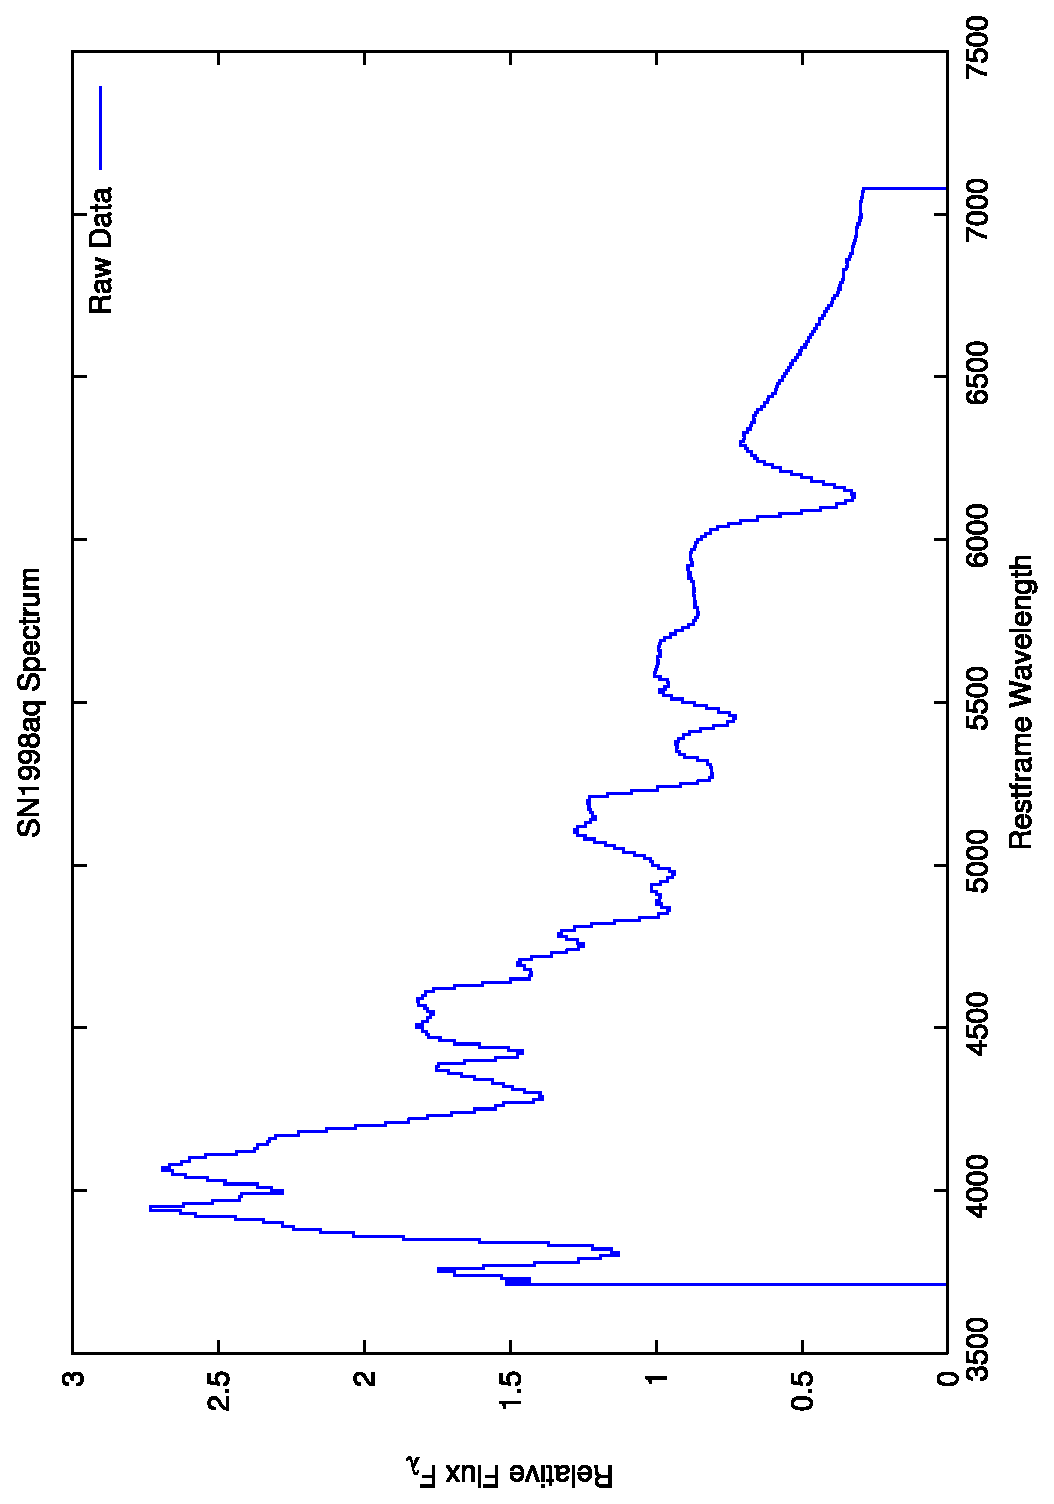
\includegraphics[angle=-90,width=0.8\textwidth]{./figures/spectrabeforeafter/SN1998aq_handpicked_v001_v027_before_after_spectra.ps}
\hfill
\includegraphics[angle=-90,width=0.8\textwidth]{./figures/corrections/SN1998aq_v001_correction.ps}
\hfill
\caption{SN1998aq spectrum before and after warping, as well as the correction function used to warp.}
\label{fig:SN1998aqfour1}
\end{figure}

\clearpage

\begin{figure}[p]
\centering
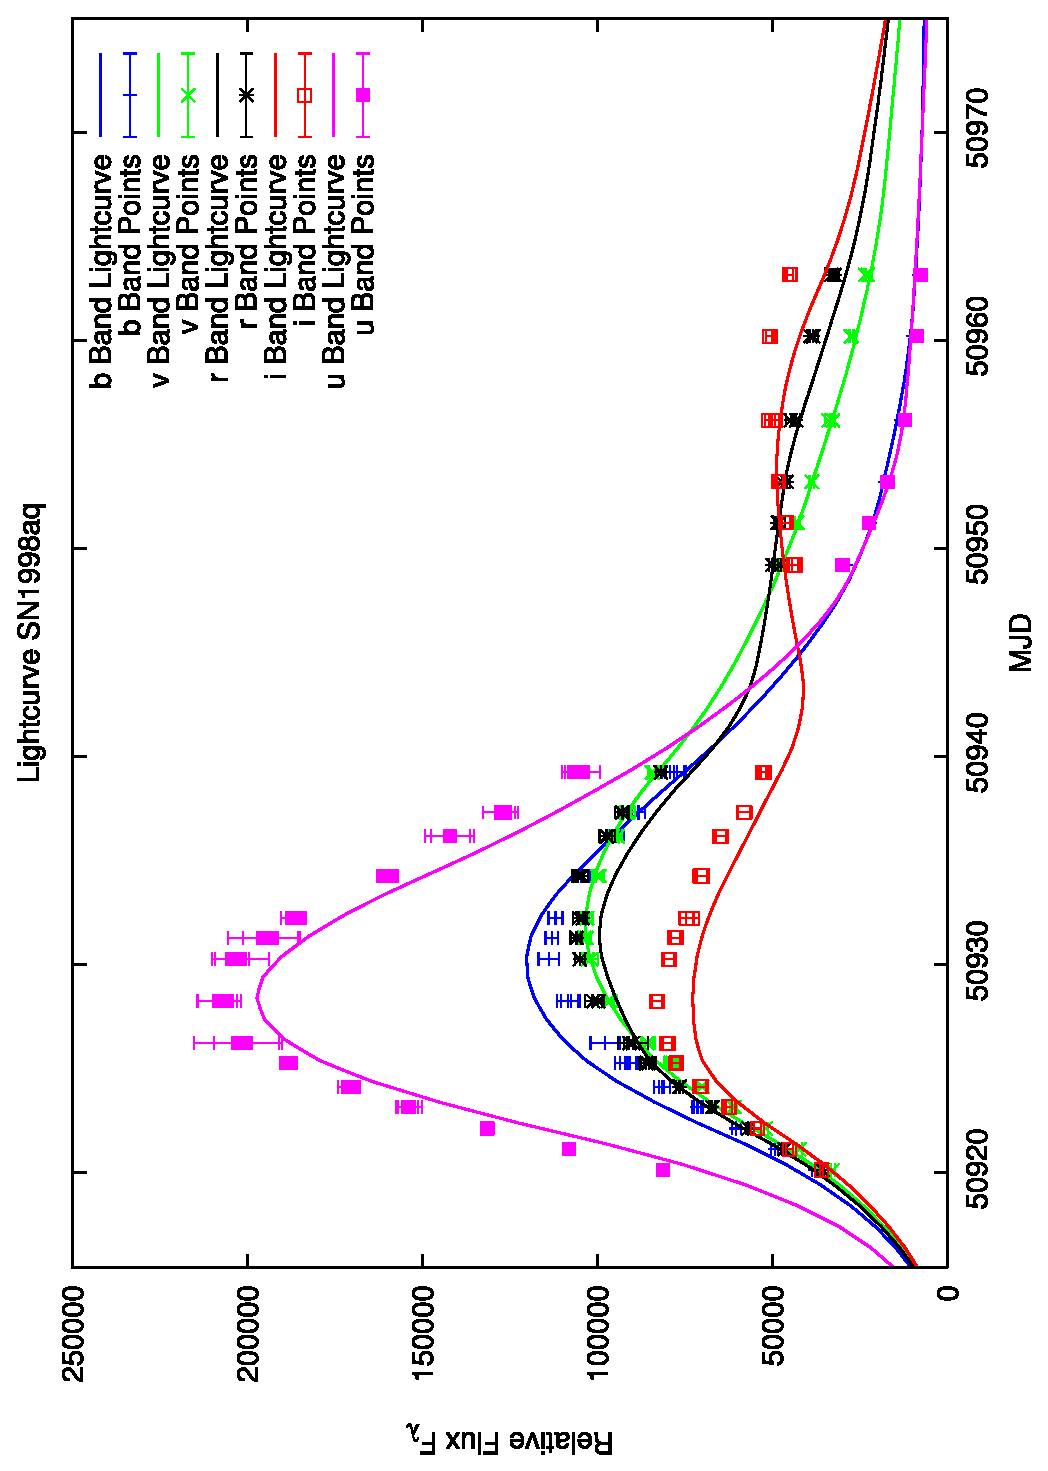
\includegraphics[angle=-90,width=0.8\textwidth]{./figures/ltcv/SN1998aq_v027_lightcurve.ps}
\hfill
\includegraphics[angle=-90,width=0.8\textwidth]{./figures/hsiao/SN1998aq_v001_hsiao.ps}
\hfill
\caption{SN1998aq light curve fit, as well as the best fit for Hsiao template warped using the Cardelli law to match the spectrum.}
\label{fig:SN1998aqfour2}
\end{figure}

\clearpage

\begin{figure}[p]
\centering
\includegraphics[angle=-90,width=0.8\textwidth]{./figures/spectrabeforeafter/SN1998bp_handpicked_v001_v027_before_after_spectra.ps}
\hfill
\includegraphics[angle=-90,width=0.8\textwidth]{./figures/corrections/SN1998bp_v001_correction.ps}
\hfill
\caption{SN1998bp spectrum before and after warping, as well as the correction function used to warp.}
\label{fig:SN1998bpfour1}
\end{figure}

\clearpage

\begin{figure}[p]
\centering
\includegraphics[angle=-90,width=0.8\textwidth]{./figures/ltcv/SN1998bp_v027_lightcurve.ps}
\hfill
\includegraphics[angle=-90,width=0.8\textwidth]{./figures/hsiao/SN1998bp_v001_hsiao.ps}
\hfill
\caption{SN1998bp light curve fit, as well as the best fit for Hsiao template warped using the Cardelli law to match the spectrum.}
\label{fig:SN1998bpfour2}
\end{figure}

\clearpage

\begin{figure}[p]
\centering
\includegraphics[angle=-90,width=0.8\textwidth]{./figures/spectrabeforeafter/SN1998de_handpicked_v001_v023_before_after_spectra.ps}
\hfill
\includegraphics[angle=-90,width=0.8\textwidth]{./figures/corrections/SN1998de_v001_correction.ps}
\hfill
\caption{SN1998de spectrum before and after warping, as well as the correction function used to warp.}
\label{fig:SN1998defour1}
\end{figure}

\clearpage

\begin{figure}[p]
\centering
\includegraphics[angle=-90,width=0.8\textwidth]{./figures/ltcv/SN1998de_v023_lightcurve.ps}
\hfill
\includegraphics[angle=-90,width=0.8\textwidth]{./figures/hsiao/SN1998de_v001_hsiao.ps}
\hfill
\caption{SN1998de light curve fit, as well as the best fit for Hsiao template warped using the Cardelli law to match the spectrum.}
\label{fig:SN1998defour2}
\end{figure}

\clearpage

\begin{figure}[p]
\centering
\includegraphics[angle=-90,width=0.8\textwidth]{./figures/spectrabeforeafter/SN1998dh_handpicked_v001_v027_before_after_spectra.ps}
\hfill
\includegraphics[angle=-90,width=0.8\textwidth]{./figures/corrections/SN1998dh_v001_correction.ps}
\hfill
\caption{SN1998dh spectrum before and after warping, as well as the correction function used to warp.}
\label{fig:SN1998dhfour1}
\end{figure}

\clearpage

\begin{figure}[p]
\centering
\includegraphics[angle=-90,width=0.8\textwidth]{./figures/ltcv/SN1998dh_v027_lightcurve.ps}
\hfill
\includegraphics[angle=-90,width=0.8\textwidth]{./figures/hsiao/SN1998dh_v001_hsiao.ps}
\hfill
\caption{SN1998dh light curve fit, as well as the best fit for Hsiao template warped using the Cardelli law to match the spectrum.}
\label{fig:SN1998dhfour2}
\end{figure}

\clearpage

\begin{figure}[p]
\centering
\includegraphics[angle=-90,width=0.8\textwidth]{./figures/spectrabeforeafter/SN1998ec_handpicked_v001_v027_before_after_spectra.ps}
\hfill
\includegraphics[angle=-90,width=0.8\textwidth]{./figures/corrections/SN1998ec_v001_correction.ps}
\hfill
\caption{SN1998ec spectrum before and after warping, as well as the correction function used to warp.}
\label{fig:SN1998ecfour1}
\end{figure}

\clearpage

\begin{figure}[p]
\centering
\includegraphics[angle=-90,width=0.8\textwidth]{./figures/ltcv/SN1998ec_v027_lightcurve.ps}
\hfill
\includegraphics[angle=-90,width=0.8\textwidth]{./figures/hsiao/SN1998ec_v001_hsiao.ps}
\hfill
\caption{SN1998ec light curve fit, as well as the best fit for Hsiao template warped using the Cardelli law to match the spectrum.}
\label{fig:SN1998ecfour2}
\end{figure}

\clearpage

\begin{figure}[p]
\centering
\includegraphics[angle=-90,width=0.8\textwidth]{./figures/spectrabeforeafter/SN1998eg_handpicked_v001_v023_before_after_spectra.ps}
\hfill
\includegraphics[angle=-90,width=0.8\textwidth]{./figures/corrections/SN1998eg_v001_correction.ps}
\hfill
\caption{SN1998eg spectrum before and after warping, as well as the correction function used to warp.}
\label{fig:SN1998egfour1}
\end{figure}

\clearpage

\begin{figure}[p]
\centering
\includegraphics[angle=-90,width=0.8\textwidth]{./figures/ltcv/SN1998eg_v023_lightcurve.ps}
\hfill
\includegraphics[angle=-90,width=0.8\textwidth]{./figures/hsiao/SN1998eg_v001_hsiao.ps}
\hfill
\caption{SN1998eg light curve fit, as well as the best fit for Hsiao template warped using the Cardelli law to match the spectrum.}
\label{fig:SN1998egfour2}
\end{figure}

\clearpage

\begin{figure}[p]
\centering
\includegraphics[angle=-90,width=0.8\textwidth]{./figures/spectrabeforeafter/SN1998es_handpicked_v001_v024_before_after_spectra.ps}
\hfill
\includegraphics[angle=-90,width=0.8\textwidth]{./figures/corrections/SN1998es_v001_correction.ps}
\hfill
\caption{SN1998es spectrum before and after warping, as well as the correction function used to warp.}
\label{fig:SN1998esfour1}
\end{figure}

\clearpage

\begin{figure}[p]
\centering
\includegraphics[angle=-90,width=0.8\textwidth]{./figures/ltcv/SN1998es_v024_lightcurve.ps}
\hfill
\includegraphics[angle=-90,width=0.8\textwidth]{./figures/hsiao/SN1998es_v001_hsiao.ps}
\hfill
\caption{SN1998es light curve fit, as well as the best fit for Hsiao template warped using the Cardelli law to match the spectrum.}
\label{fig:SN1998esfour2}
\end{figure}

\clearpage

\begin{figure}[p]
\centering
\includegraphics[angle=-90,width=0.8\textwidth]{./figures/spectrabeforeafter/SN1999aa_handpicked_v001_v023_before_after_spectra.ps}
\hfill
\includegraphics[angle=-90,width=0.8\textwidth]{./figures/corrections/SN1999aa_v001_correction.ps}
\hfill
\caption{SN1999aa spectrum before and after warping, as well as the correction function used to warp.}
\label{fig:SN1999aafour1}
\end{figure}

\clearpage

\begin{figure}[p]
\centering
\includegraphics[angle=-90,width=0.8\textwidth]{./figures/ltcv/SN1999aa_v023_lightcurve.ps}
\hfill
\includegraphics[angle=-90,width=0.8\textwidth]{./figures/hsiao/SN1999aa_v001_hsiao.ps}
\hfill
\caption{SN1999aa light curve fit, as well as the best fit for Hsiao template warped using the Cardelli law to match the spectrum.}
\label{fig:SN1999aafour2}
\end{figure}

\clearpage

\begin{figure}[p]
\centering
\includegraphics[angle=-90,width=0.8\textwidth]{./figures/spectrabeforeafter/SN1999ac_handpicked_v001_v024_before_after_spectra.ps}
\hfill
\includegraphics[angle=-90,width=0.8\textwidth]{./figures/corrections/SN1999ac_v001_correction.ps}
\hfill
\caption{SN1999ac spectrum before and after warping, as well as the correction function used to warp.}
\label{fig:SN1999acfour1}
\end{figure}

\clearpage

\begin{figure}[p]
\centering
\includegraphics[angle=-90,width=0.8\textwidth]{./figures/ltcv/SN1999ac_v024_lightcurve.ps}
\hfill
\includegraphics[angle=-90,width=0.8\textwidth]{./figures/hsiao/SN1999ac_v001_hsiao.ps}
\hfill
\caption{SN1999ac light curve fit, as well as the best fit for Hsiao template warped using the Cardelli law to match the spectrum.}
\label{fig:SN1999acfour2}
\end{figure}

\clearpage

\begin{figure}[p]
\centering
\includegraphics[angle=-90,width=0.8\textwidth]{./figures/spectrabeforeafter/SN1999cc_handpicked_v001_v027_before_after_spectra.ps}
\hfill
\includegraphics[angle=-90,width=0.8\textwidth]{./figures/corrections/SN1999cc_v001_correction.ps}
\hfill
\caption{SN1999cc spectrum before and after warping, as well as the correction function used to warp.}
\label{fig:SN1999ccfour1}
\end{figure}

\clearpage

\begin{figure}[p]
\centering
\includegraphics[angle=-90,width=0.8\textwidth]{./figures/ltcv/SN1999cc_v027_lightcurve.ps}
\hfill
\includegraphics[angle=-90,width=0.8\textwidth]{./figures/hsiao/SN1999cc_v001_hsiao.ps}
\hfill
\caption{SN1999cc light curve fit, as well as the best fit for Hsiao template warped using the Cardelli law to match the spectrum.}
\label{fig:SN1999ccfour2}
\end{figure}

\clearpage

\begin{figure}[p]
\centering
\includegraphics[angle=-90,width=0.8\textwidth]{./figures/spectrabeforeafter/SN1999cl_handpicked_v001_v024_before_after_spectra.ps}
\hfill
\includegraphics[angle=-90,width=0.8\textwidth]{./figures/corrections/SN1999cl_v001_correction.ps}
\hfill
\caption{SN1999cl spectrum before and after warping, as well as the correction function used to warp.}
\label{fig:SN1999clfour1}
\end{figure}

\clearpage

\begin{figure}[p]
\centering
\includegraphics[angle=-90,width=0.8\textwidth]{./figures/ltcv/SN1999cl_v024_lightcurve.ps}
\hfill
\includegraphics[angle=-90,width=0.8\textwidth]{./figures/hsiao/SN1999cl_v001_hsiao.ps}
\hfill
\caption{SN1999cl light curve fit, as well as the best fit for Hsiao template warped using the Cardelli law to match the spectrum.}
\label{fig:SN1999clfour2}
\end{figure}

\clearpage

\begin{figure}[p]
\centering
\includegraphics[angle=-90,width=0.8\textwidth]{./figures/spectrabeforeafter/SN1999dq_handpicked_v001_v023_before_after_spectra.ps}
\hfill
\includegraphics[angle=-90,width=0.8\textwidth]{./figures/corrections/SN1999dq_v001_correction.ps}
\hfill
\caption{SN1999dq spectrum before and after warping, as well as the correction function used to warp.}
\label{fig:SN1999dqfour1}
\end{figure}

\clearpage

\begin{figure}[p]
\centering
\includegraphics[angle=-90,width=0.8\textwidth]{./figures/ltcv/SN1999dq_v023_lightcurve.ps}
\hfill
\includegraphics[angle=-90,width=0.8\textwidth]{./figures/hsiao/SN1999dq_v001_hsiao.ps}
\hfill
\caption{SN1999dq light curve fit, as well as the best fit for Hsiao template warped using the Cardelli law to match the spectrum.}
\label{fig:SN1999dqfour2}
\end{figure}

\clearpage

\begin{figure}[p]
\centering
\includegraphics[angle=-90,width=0.8\textwidth]{./figures/spectrabeforeafter/SN1999ej_handpicked_v001_v027_before_after_spectra.ps}
\hfill
\includegraphics[angle=-90,width=0.8\textwidth]{./figures/corrections/SN1999ej_v001_correction.ps}
\hfill
\caption{SN1999ej spectrum before and after warping, as well as the correction function used to warp.}
\label{fig:SN1999ejfour1}
\end{figure}

\clearpage

\begin{figure}[p]
\centering
\includegraphics[angle=-90,width=0.8\textwidth]{./figures/ltcv/SN1999ej_v027_lightcurve.ps}
\hfill
\includegraphics[angle=-90,width=0.8\textwidth]{./figures/hsiao/SN1999ej_v001_hsiao.ps}
\hfill
\caption{SN1999ej light curve fit, as well as the best fit for Hsiao template warped using the Cardelli law to match the spectrum.}
\label{fig:SN1999ejfour2}
\end{figure}

\clearpage

\begin{figure}[p]
\centering
\includegraphics[angle=-90,width=0.8\textwidth]{./figures/spectrabeforeafter/SN1999gd_handpicked_v001_v027_before_after_spectra.ps}
\hfill
\includegraphics[angle=-90,width=0.8\textwidth]{./figures/corrections/SN1999gd_v001_correction.ps}
\hfill
\caption{SN1999gd spectrum before and after warping, as well as the correction function used to warp.}
\label{fig:SN1999gdfour1}
\end{figure}

\clearpage

\begin{figure}[p]
\centering
\includegraphics[angle=-90,width=0.8\textwidth]{./figures/ltcv/SN1999gd_v027_lightcurve.ps}
\hfill
\includegraphics[angle=-90,width=0.8\textwidth]{./figures/hsiao/SN1999gd_v001_hsiao.ps}
\hfill
\caption{SN1999gd light curve fit, as well as the best fit for Hsiao template warped using the Cardelli law to match the spectrum.}
\label{fig:SN1999gdfour2}
\end{figure}

\clearpage

\begin{figure}[p]
\centering
\includegraphics[angle=-90,width=0.8\textwidth]{./figures/spectrabeforeafter/SN1999gp_handpicked_v001_v024_before_after_spectra.ps}
\hfill
\includegraphics[angle=-90,width=0.8\textwidth]{./figures/corrections/SN1999gp_v001_correction.ps}
\hfill
\caption{SN1999gp spectrum before and after warping, as well as the correction function used to warp.}
\label{fig:SN1999gpfour1}
\end{figure}

\clearpage

\begin{figure}[p]
\centering
\includegraphics[angle=-90,width=0.8\textwidth]{./figures/ltcv/SN1999gp_v024_lightcurve.ps}
\hfill
\includegraphics[angle=-90,width=0.8\textwidth]{./figures/hsiao/SN1999gp_v001_hsiao.ps}
\hfill
\caption{SN1999gp light curve fit, as well as the best fit for Hsiao template warped using the Cardelli law to match the spectrum.}
\label{fig:SN1999gpfour2}
\end{figure}

\clearpage

\begin{figure}[p]
\centering
\includegraphics[angle=-90,width=0.8\textwidth]{./figures/spectrabeforeafter/SN2000cf_handpicked_v001_v027_before_after_spectra.ps}
\hfill
\includegraphics[angle=-90,width=0.8\textwidth]{./figures/corrections/SN2000cf_v001_correction.ps}
\hfill
\caption{SN2000cf spectrum before and after warping, as well as the correction function used to warp.}
\label{fig:SN2000cffour1}
\end{figure}

\clearpage

\begin{figure}[p]
\centering
\includegraphics[angle=-90,width=0.8\textwidth]{./figures/ltcv/SN2000cf_v027_lightcurve.ps}
\hfill
\includegraphics[angle=-90,width=0.8\textwidth]{./figures/hsiao/SN2000cf_v001_hsiao.ps}
\hfill
\caption{SN2000cf light curve fit, as well as the best fit for Hsiao template warped using the Cardelli law to match the spectrum.}
\label{fig:SN2000cffour2}
\end{figure}

\clearpage

\begin{figure}[p]
\centering
\includegraphics[angle=-90,width=0.8\textwidth]{./figures/spectrabeforeafter/SN2000cx_handpicked_v001_v024_before_after_spectra.ps}
\hfill
\includegraphics[angle=-90,width=0.8\textwidth]{./figures/corrections/SN2000cx_v001_correction.ps}
\hfill
\caption{SN2000cx spectrum before and after warping, as well as the correction function used to warp.}
\label{fig:SN2000cxfour1}
\end{figure}

\clearpage

\begin{figure}[p]
\centering
\includegraphics[angle=-90,width=0.8\textwidth]{./figures/ltcv/SN2000cx_v024_lightcurve.ps}
\hfill
\includegraphics[angle=-90,width=0.8\textwidth]{./figures/hsiao/SN2000cx_v001_hsiao.ps}
\hfill
\caption{SN2000cx light curve fit, as well as the best fit for Hsiao template warped using the Cardelli law to match the spectrum.}
\label{fig:SN2000cxfour2}
\end{figure}

\clearpage

\begin{figure}[p]
\centering
\includegraphics[angle=-90,width=0.8\textwidth]{./figures/spectrabeforeafter/SN2000dk_handpicked_v001_v027_before_after_spectra.ps}
\hfill
\includegraphics[angle=-90,width=0.8\textwidth]{./figures/corrections/SN2000dk_v001_correction.ps}
\hfill
\caption{SN2000dk spectrum before and after warping, as well as the correction function used to warp.}
\label{fig:SN2000dkfour1}
\end{figure}

\clearpage

\begin{figure}[p]
\centering
\includegraphics[angle=-90,width=0.8\textwidth]{./figures/ltcv/SN2000dk_v027_lightcurve.ps}
\hfill
\includegraphics[angle=-90,width=0.8\textwidth]{./figures/hsiao/SN2000dk_v001_hsiao.ps}
\hfill
\caption{SN2000dk light curve fit, as well as the best fit for Hsiao template warped using the Cardelli law to match the spectrum.}
\label{fig:SN2000dkfour2}
\end{figure}

\clearpage

\begin{figure}[p]
\centering
\includegraphics[angle=-90,width=0.8\textwidth]{./figures/spectrabeforeafter/SN2000fa_handpicked_v001_v023_before_after_spectra.ps}
\hfill
\includegraphics[angle=-90,width=0.8\textwidth]{./figures/corrections/SN2000fa_v001_correction.ps}
\hfill
\caption{SN2000fa spectrum before and after warping, as well as the correction function used to warp.}
\label{fig:SN2000fafour1}
\end{figure}

\clearpage

\begin{figure}[p]
\centering
\includegraphics[angle=-90,width=0.8\textwidth]{./figures/ltcv/SN2000fa_v023_lightcurve.ps}
\hfill
\includegraphics[angle=-90,width=0.8\textwidth]{./figures/hsiao/SN2000fa_v001_hsiao.ps}
\hfill
\caption{SN2000fa light curve fit, as well as the best fit for Hsiao template warped using the Cardelli law to match the spectrum.}
\label{fig:SN2000fafour2}
\end{figure}

\clearpage
<<<<<<< .mine
=======

\begin{figure}[p]
\centering
\includegraphics[angle=-90,width=0.8\textwidth]{./figures/spectrabeforeafter/SN1991T.ps}
\hfill
\includegraphics[angle=-90,width=0.8\textwidth]{./figures/spectrabeforeafter/SN1991bg.ps}
\hfill
\caption{SN1991T Spectrum and SN1991bg Spectrum.}
\label{fig:SN1991}
\end{figure}
\clearpage
>>>>>>> .r1205


\end{document}
